\documentclass{beamer}
\usetheme[subsectionpage=progressbar,
		  progressbar=frametitle,
		  % background=dark
		 ]{metropolis}

\usepackage{media9}
\usepackage[spanish]{babel}
		 
\title{Taller Básico de Impresión 3D}
\date{\today}
\author{Idir Expósito Gómez}
\institute{Málaga MakerSpace}
\begin{document}
	\maketitle
	
	%%%%%%%%%%%%%%%%%%%%%%%%%%%%%%%%%%%%%%%%
	\section{Introducción}
	
	\subsection{Qué es el Málaga MakerSpace}
	
	\subsection{Objetivos de este taller}
	\begin{frame}{Competencias generales}
		\begin{itemize}
			\item Entender los principios físicos de la impresión 3D.
			\item Reconocer qué se puede fabricar con esta tecnología.
			\item Conocer las partes físicas de una impresora y su función.
			\item Conocer los principios del rebanado (slicing).
		\end{itemize}
	\end{frame}
	\begin{frame}{Competencias específicas}
		\begin{itemize}
			\item Ajustar los parámetros más importantes con Ultimaker CURA.
			\item Conocer la impresora Creality CR-10 y su calibrado.
			\item Conocer los problemas de impresión más comunes y cómo solventarlos.
			\item Conocer las reglas de impresión en el Málaga MakerSpace.
		\end{itemize}
	\end{frame}
	
	\subsection{Sistema de impresión en el MMS}
	\begin{frame}{Reglas}
		\begin{enumerate}
			\item Obligatorio superar este taller.
			\item Solo impresión con PLA y mantenimiento básico.
			\item Siempre debe haber supervisión de la impresión.
			\item No desatender la impresora si no se puede controlar remotamente.
			\item Respetar legislación de derechos de autor.
			\item Uso responsable de la maquinaria y responsabilización de los errores.
			\item Prohibido modificar la maquinaria.
			\item Obligatoria reserva de maquinaria y material.
			\item El pago se realiza por adelantado.
			\item Se pueden realizar trabajos para terceros con autorización previa.
		\end{enumerate}
	\end{frame}
	\begin{frame}[standout]{Costes}
		El sistema de costes es provisional mientras no haya cuota de membresía y espacio físico.
	\end{frame}
	\begin{frame}{Costes para personas no cualificadas}
		\begin{enumerate}
			\item 0.03€ por gramo de PLA.
			\item 0.25€ por hora de impresión, en intervalos de media hora.
			\item 5€ por hora de trabajo humano.
			\item 10\% adicional por fallos.
			\item 21\% de IVA.
		\end{enumerate}
		$$\text{Coste}=1.21\times 1.1\times \left( 5\times \text{Operario} +0.25\times\text{Horas}+0.03\times\text{Gramos} \right)$$
	\end{frame}
	\begin{frame}{Costes para personas cualificadas sin material}
		\begin{enumerate}
			\item 0.03€ por gramo de PLA.
			\item 0.25€ por hora de impresión, en intervalos de media hora.
			\item 21\% de IVA.
		\end{enumerate}
		$$\text{Coste}=1.21\times \left( 0.25\times\text{Horas}+0.03\times\text{Gramos} \right)$$
	\end{frame}
	\begin{frame}{Costes para personas cualificadas con material}
		\begin{enumerate}
			\item 0.25€ por hora de impresión, en intervalos de media hora.
			\item 21\% de IVA.
		\end{enumerate}
		$$\text{Coste}=1.21\times \left( 0.25\times\text{Horas} \right)$$
	\end{frame}
	
	%%%%%%%%%%%%%%%%%%%%%%%%%%%%%%%%%%%%%%%%
	\section{Fundamentos de Modelado por Deposición Fundida (FDM)}
	\begin{frame}{Fundamentos de FDM}
		\begin{figure}
			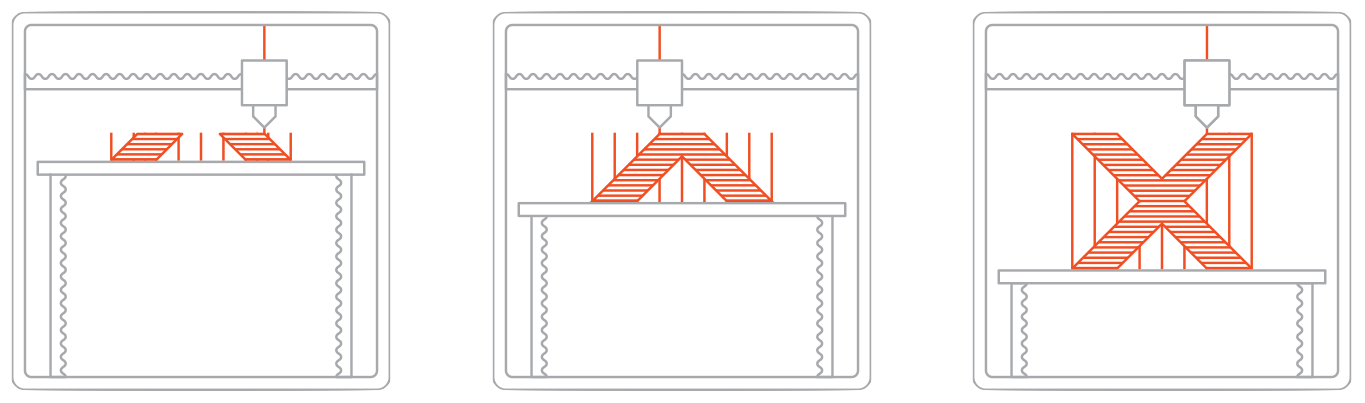
\includegraphics[width=\textwidth]{images/fdm}
			\caption{Proceso FDM}
		\end{figure}
	\end{frame}
	
	\subsection{Partes y características de una impresora}
	\begin{frame}{Placa madre y control}
		\begin{figure}
			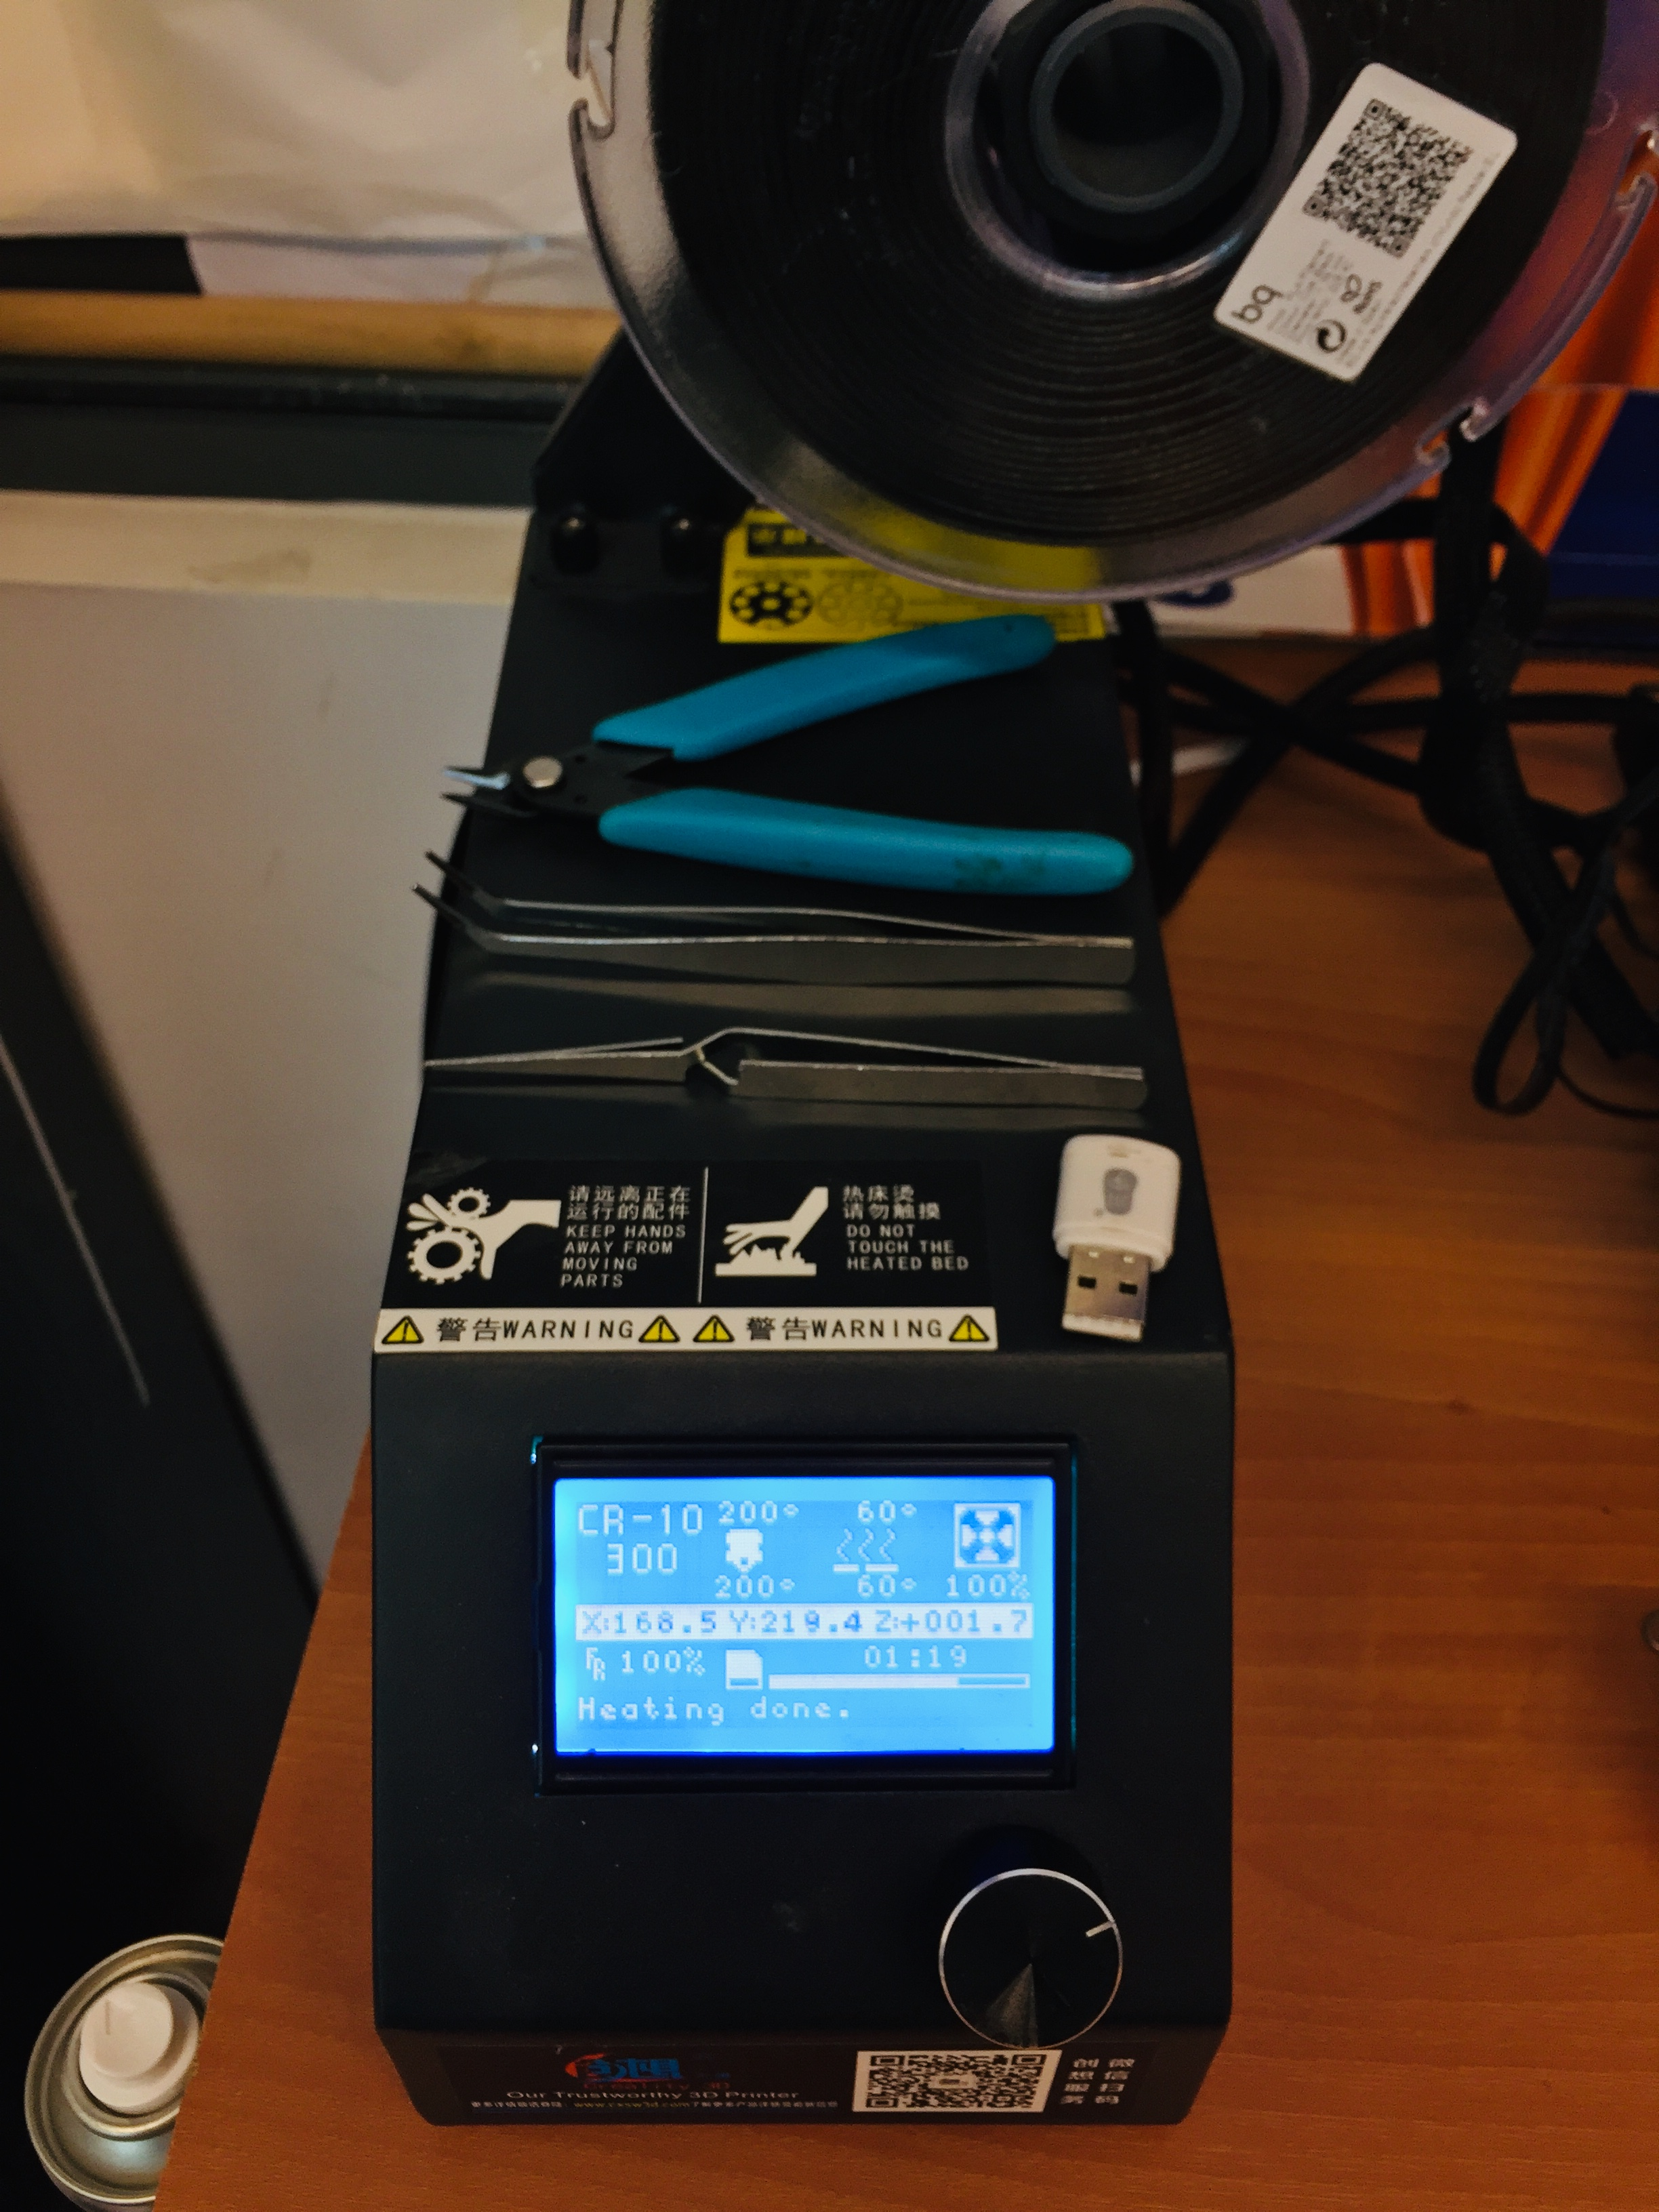
\includegraphics[height=0.8\textheight]{images/control}
			\caption{Unidad de control}
		\end{figure}
	\end{frame}
	\begin{frame}{Extrusor}
		\begin{figure}
			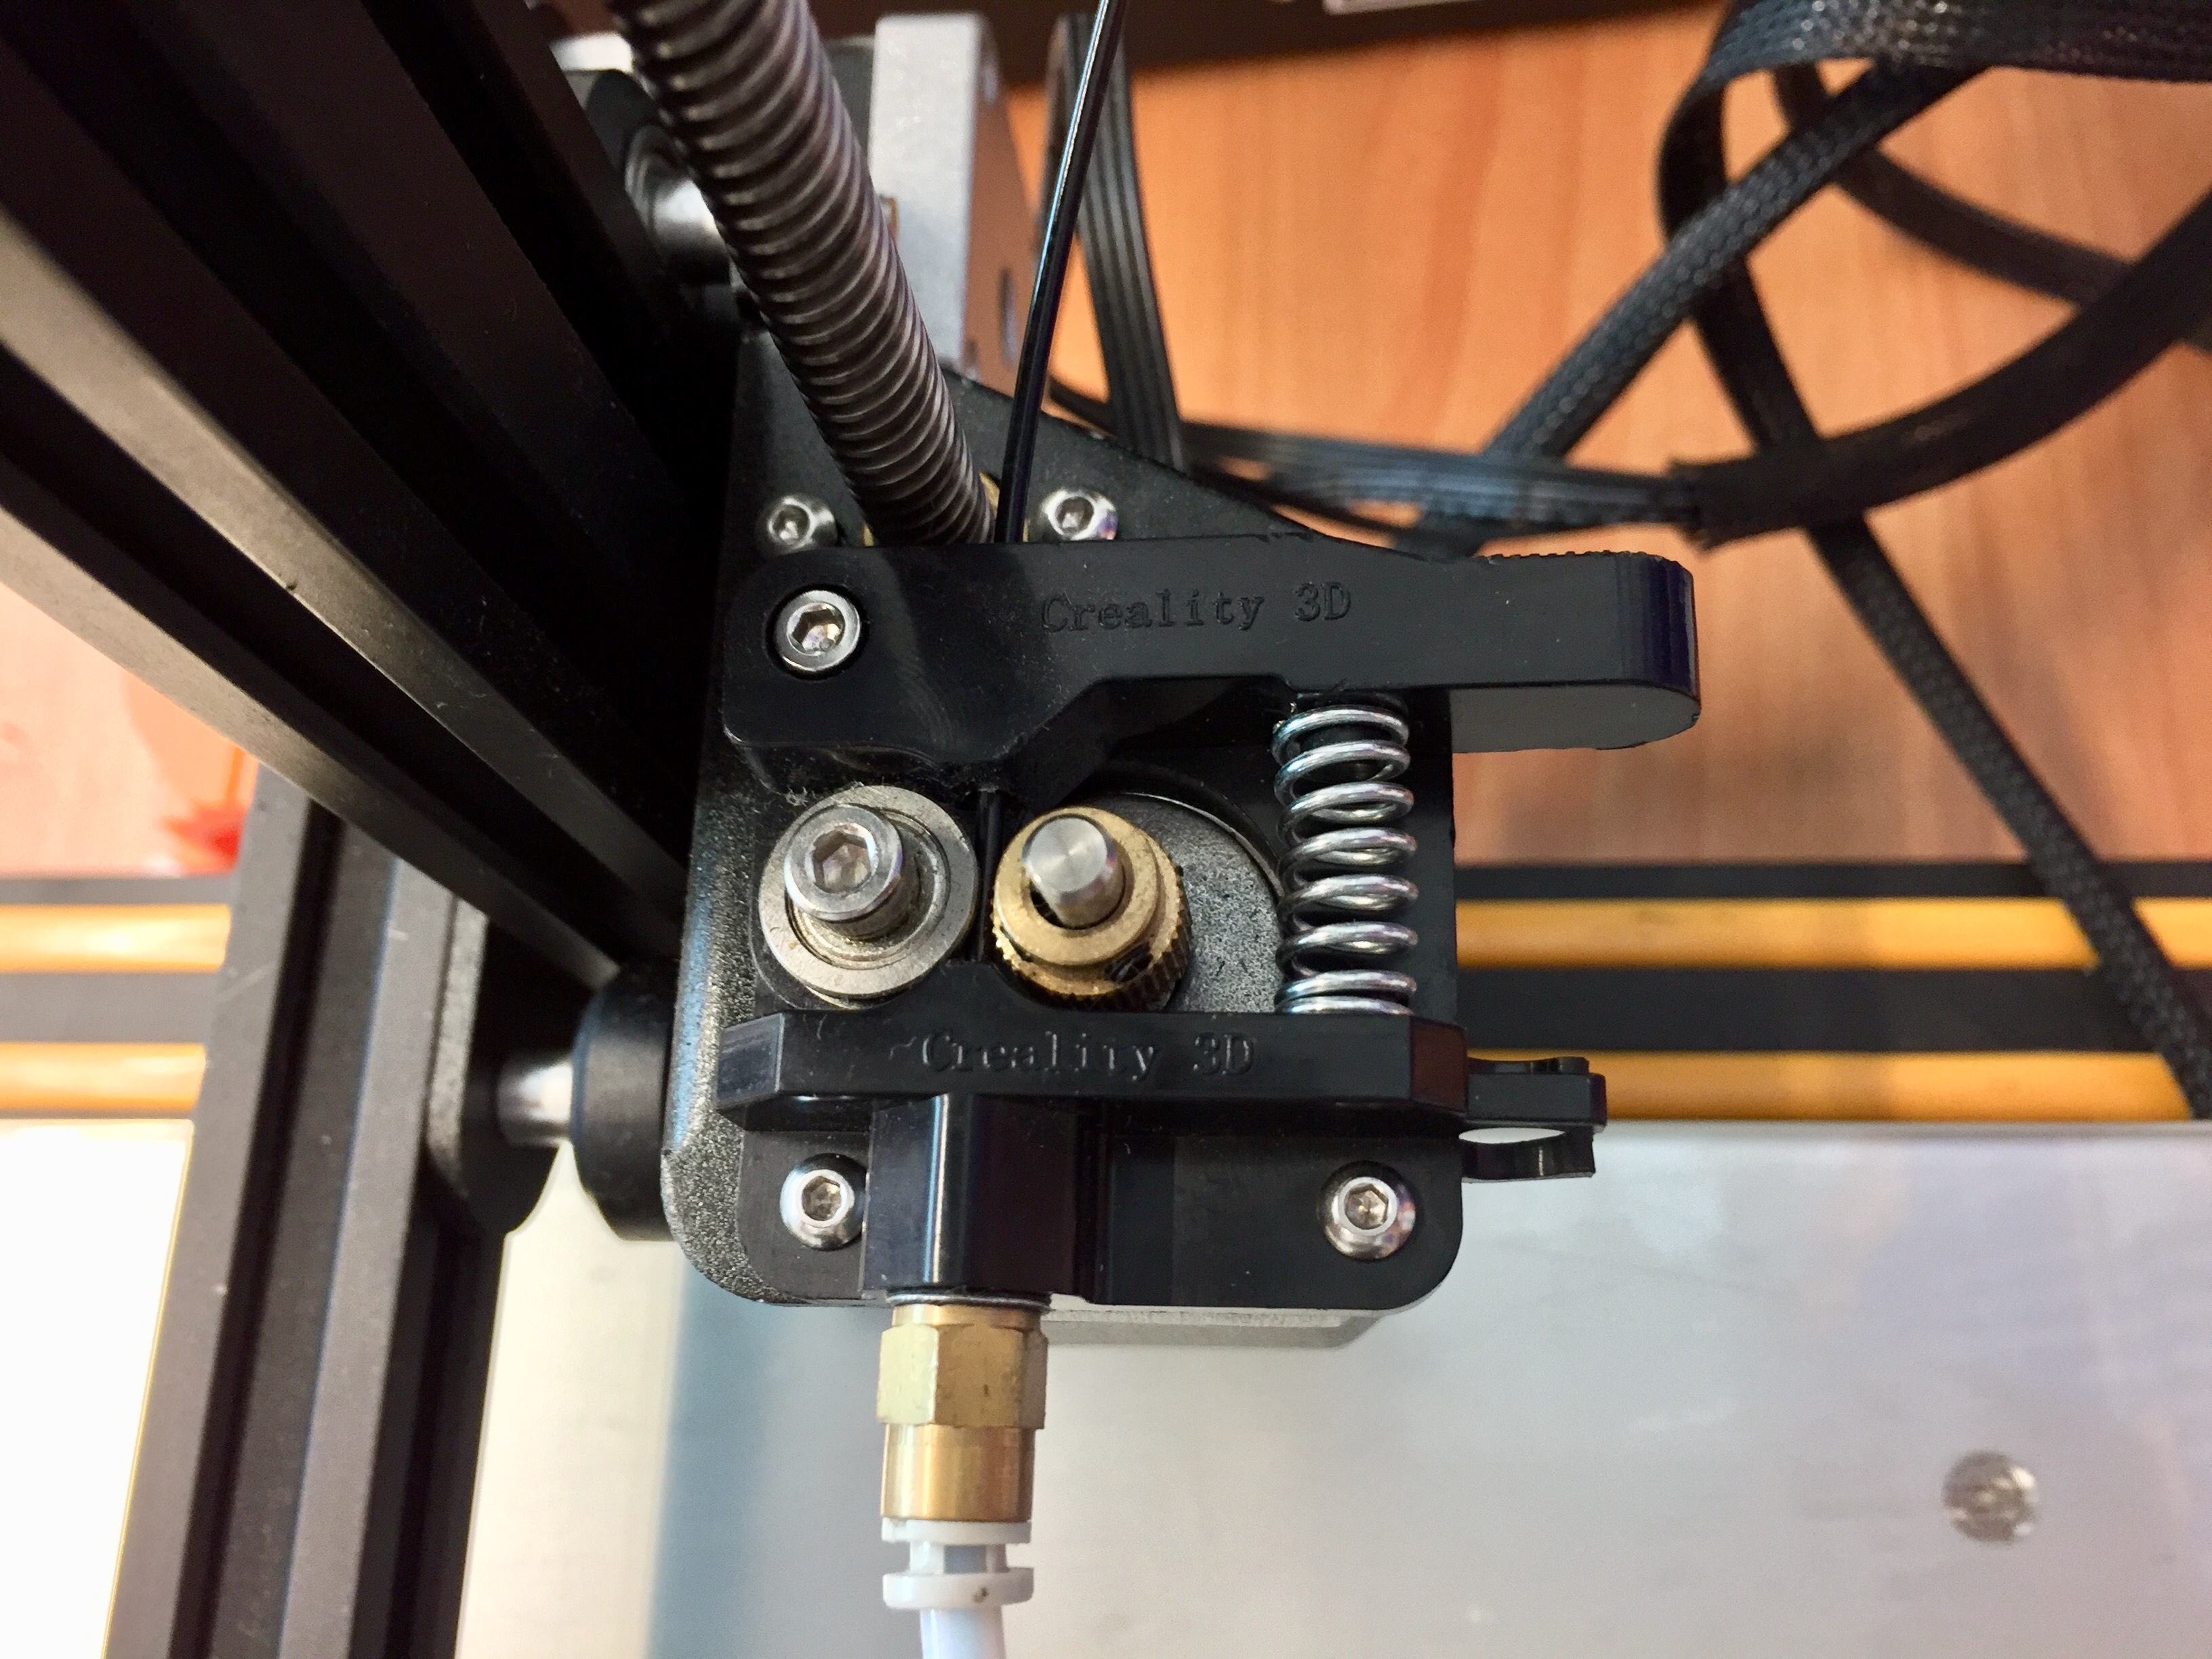
\includegraphics[height=0.8\textheight]{images/extrusor}
			\caption{Extrusor indirecto}
		\end{figure}
	\end{frame}
	\begin{frame}{Cabezal de impresión}
		\begin{figure}
			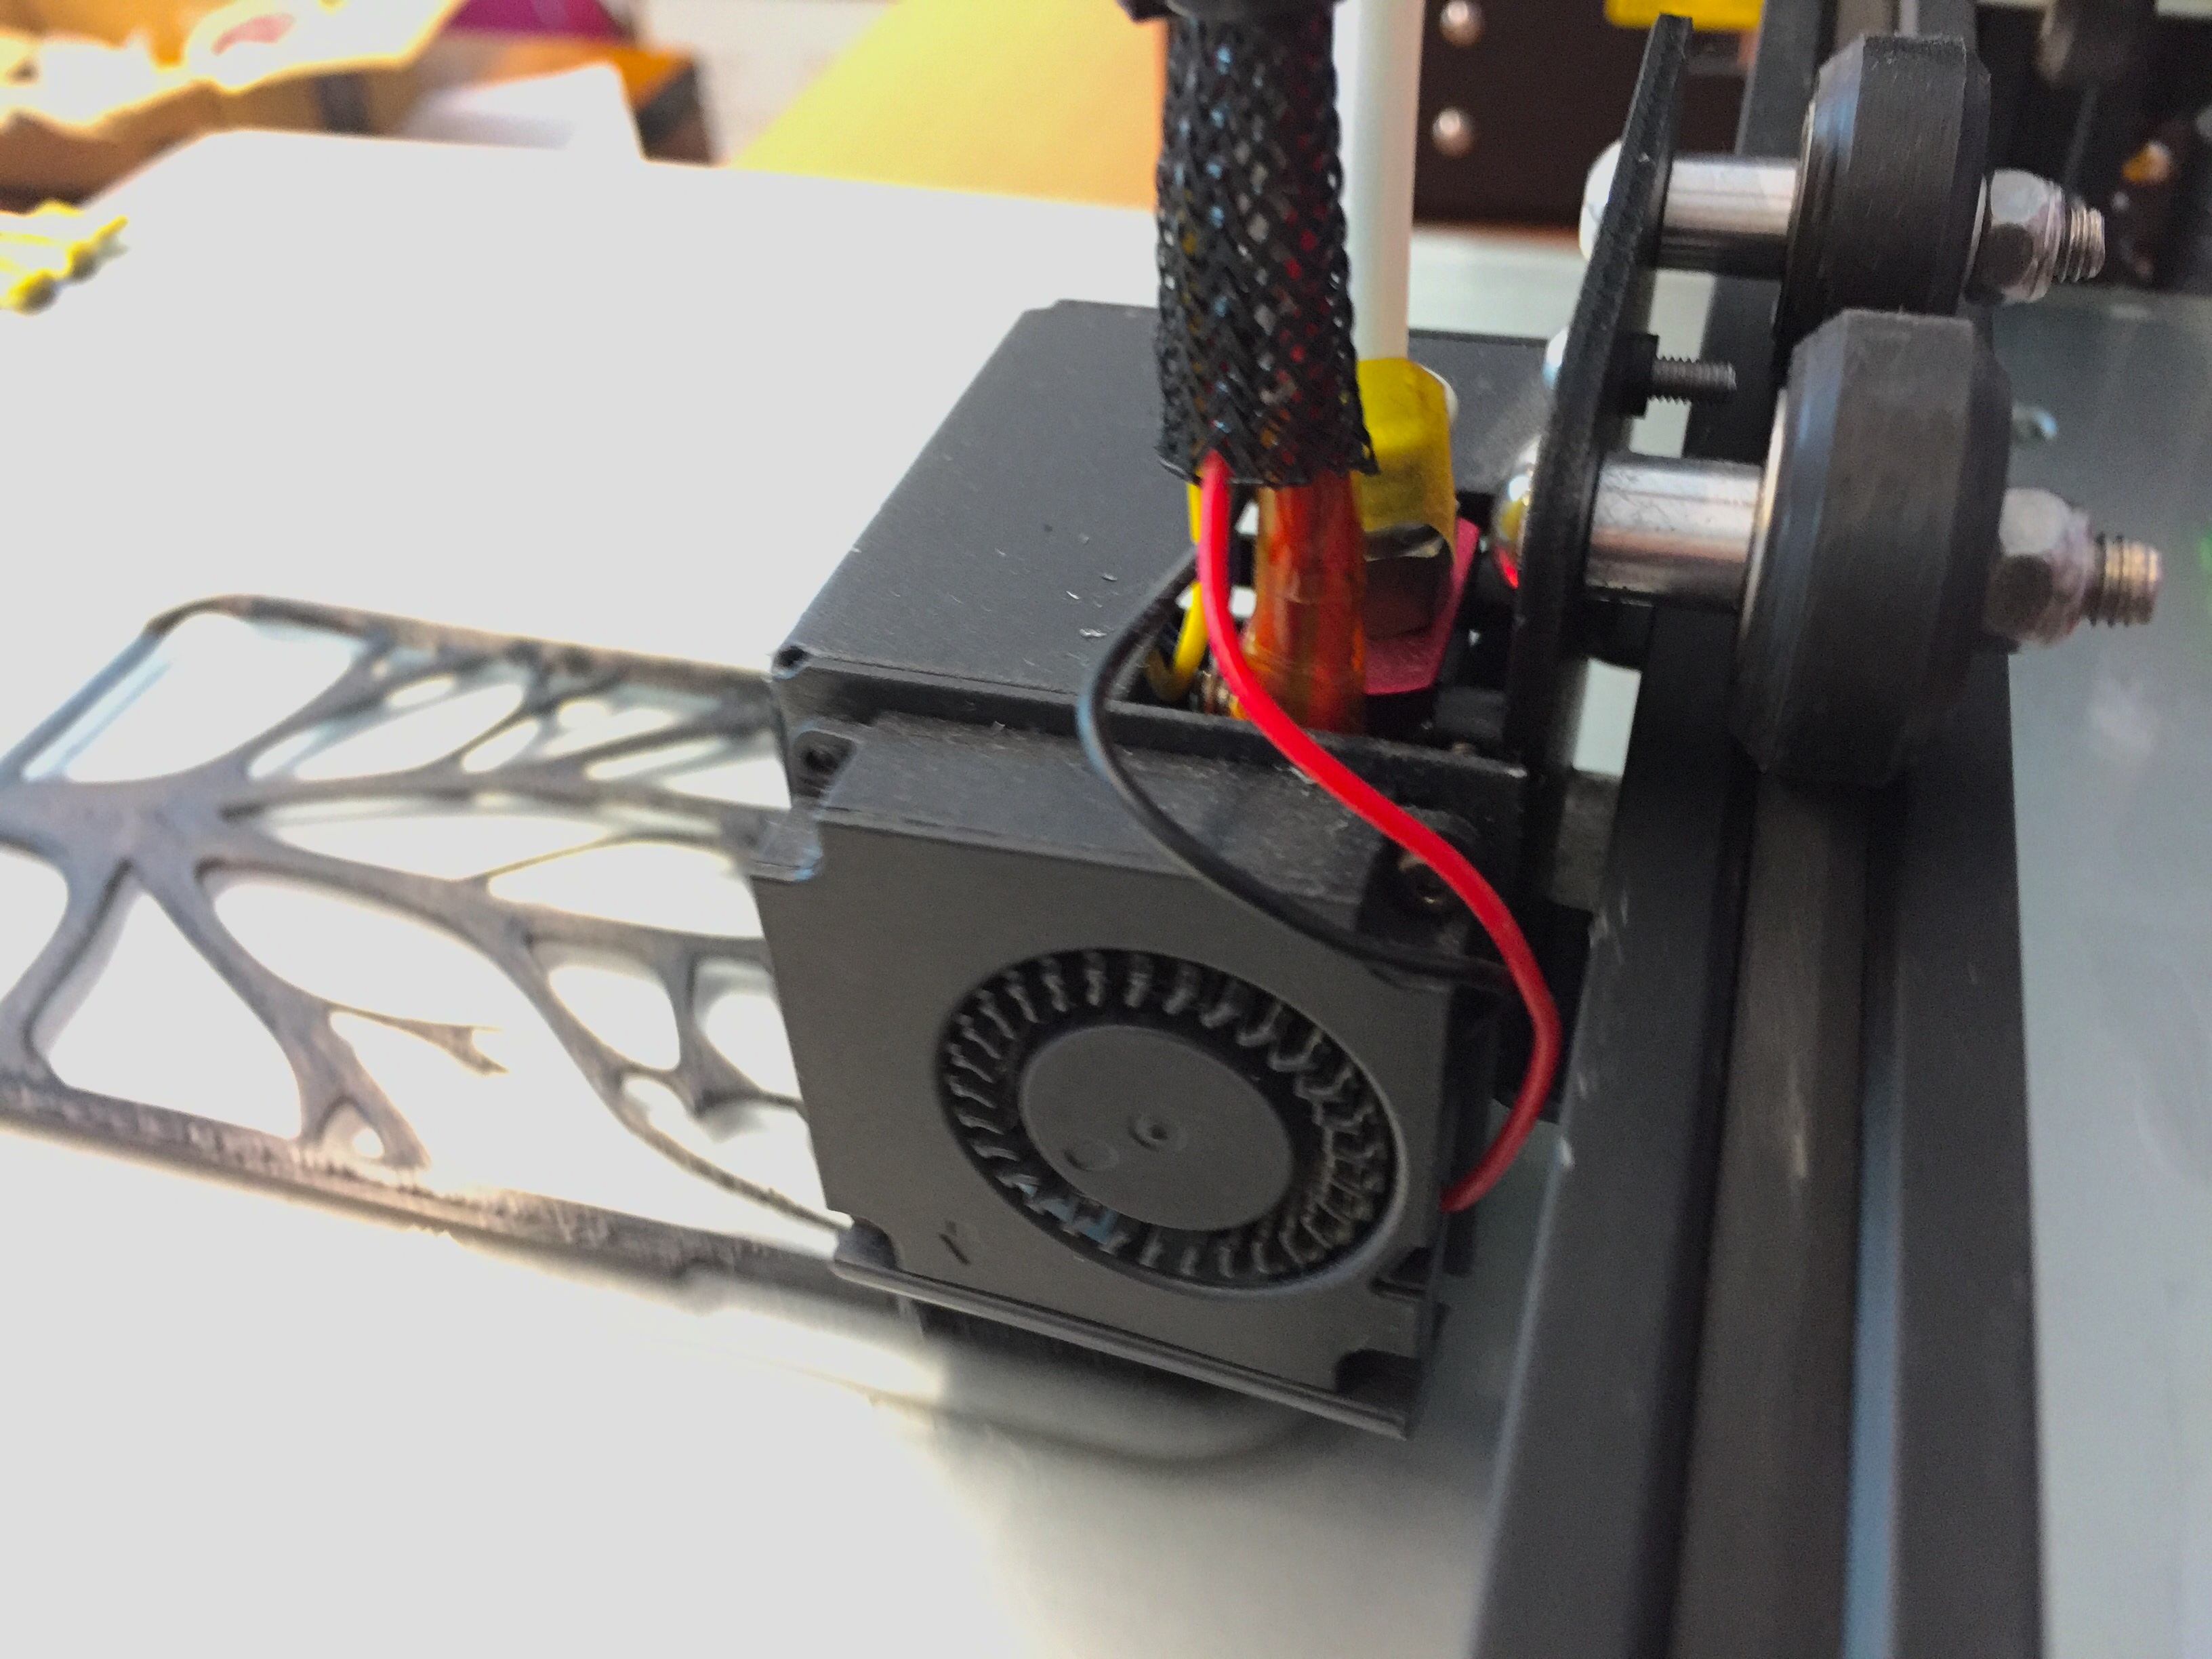
\includegraphics[height=0.8\textheight]{images/cabezal}
			\caption{Cabezal durante una impresión}
		\end{figure}
	\end{frame}
	\begin{frame}{Cama de impresión}
		\begin{figure}
			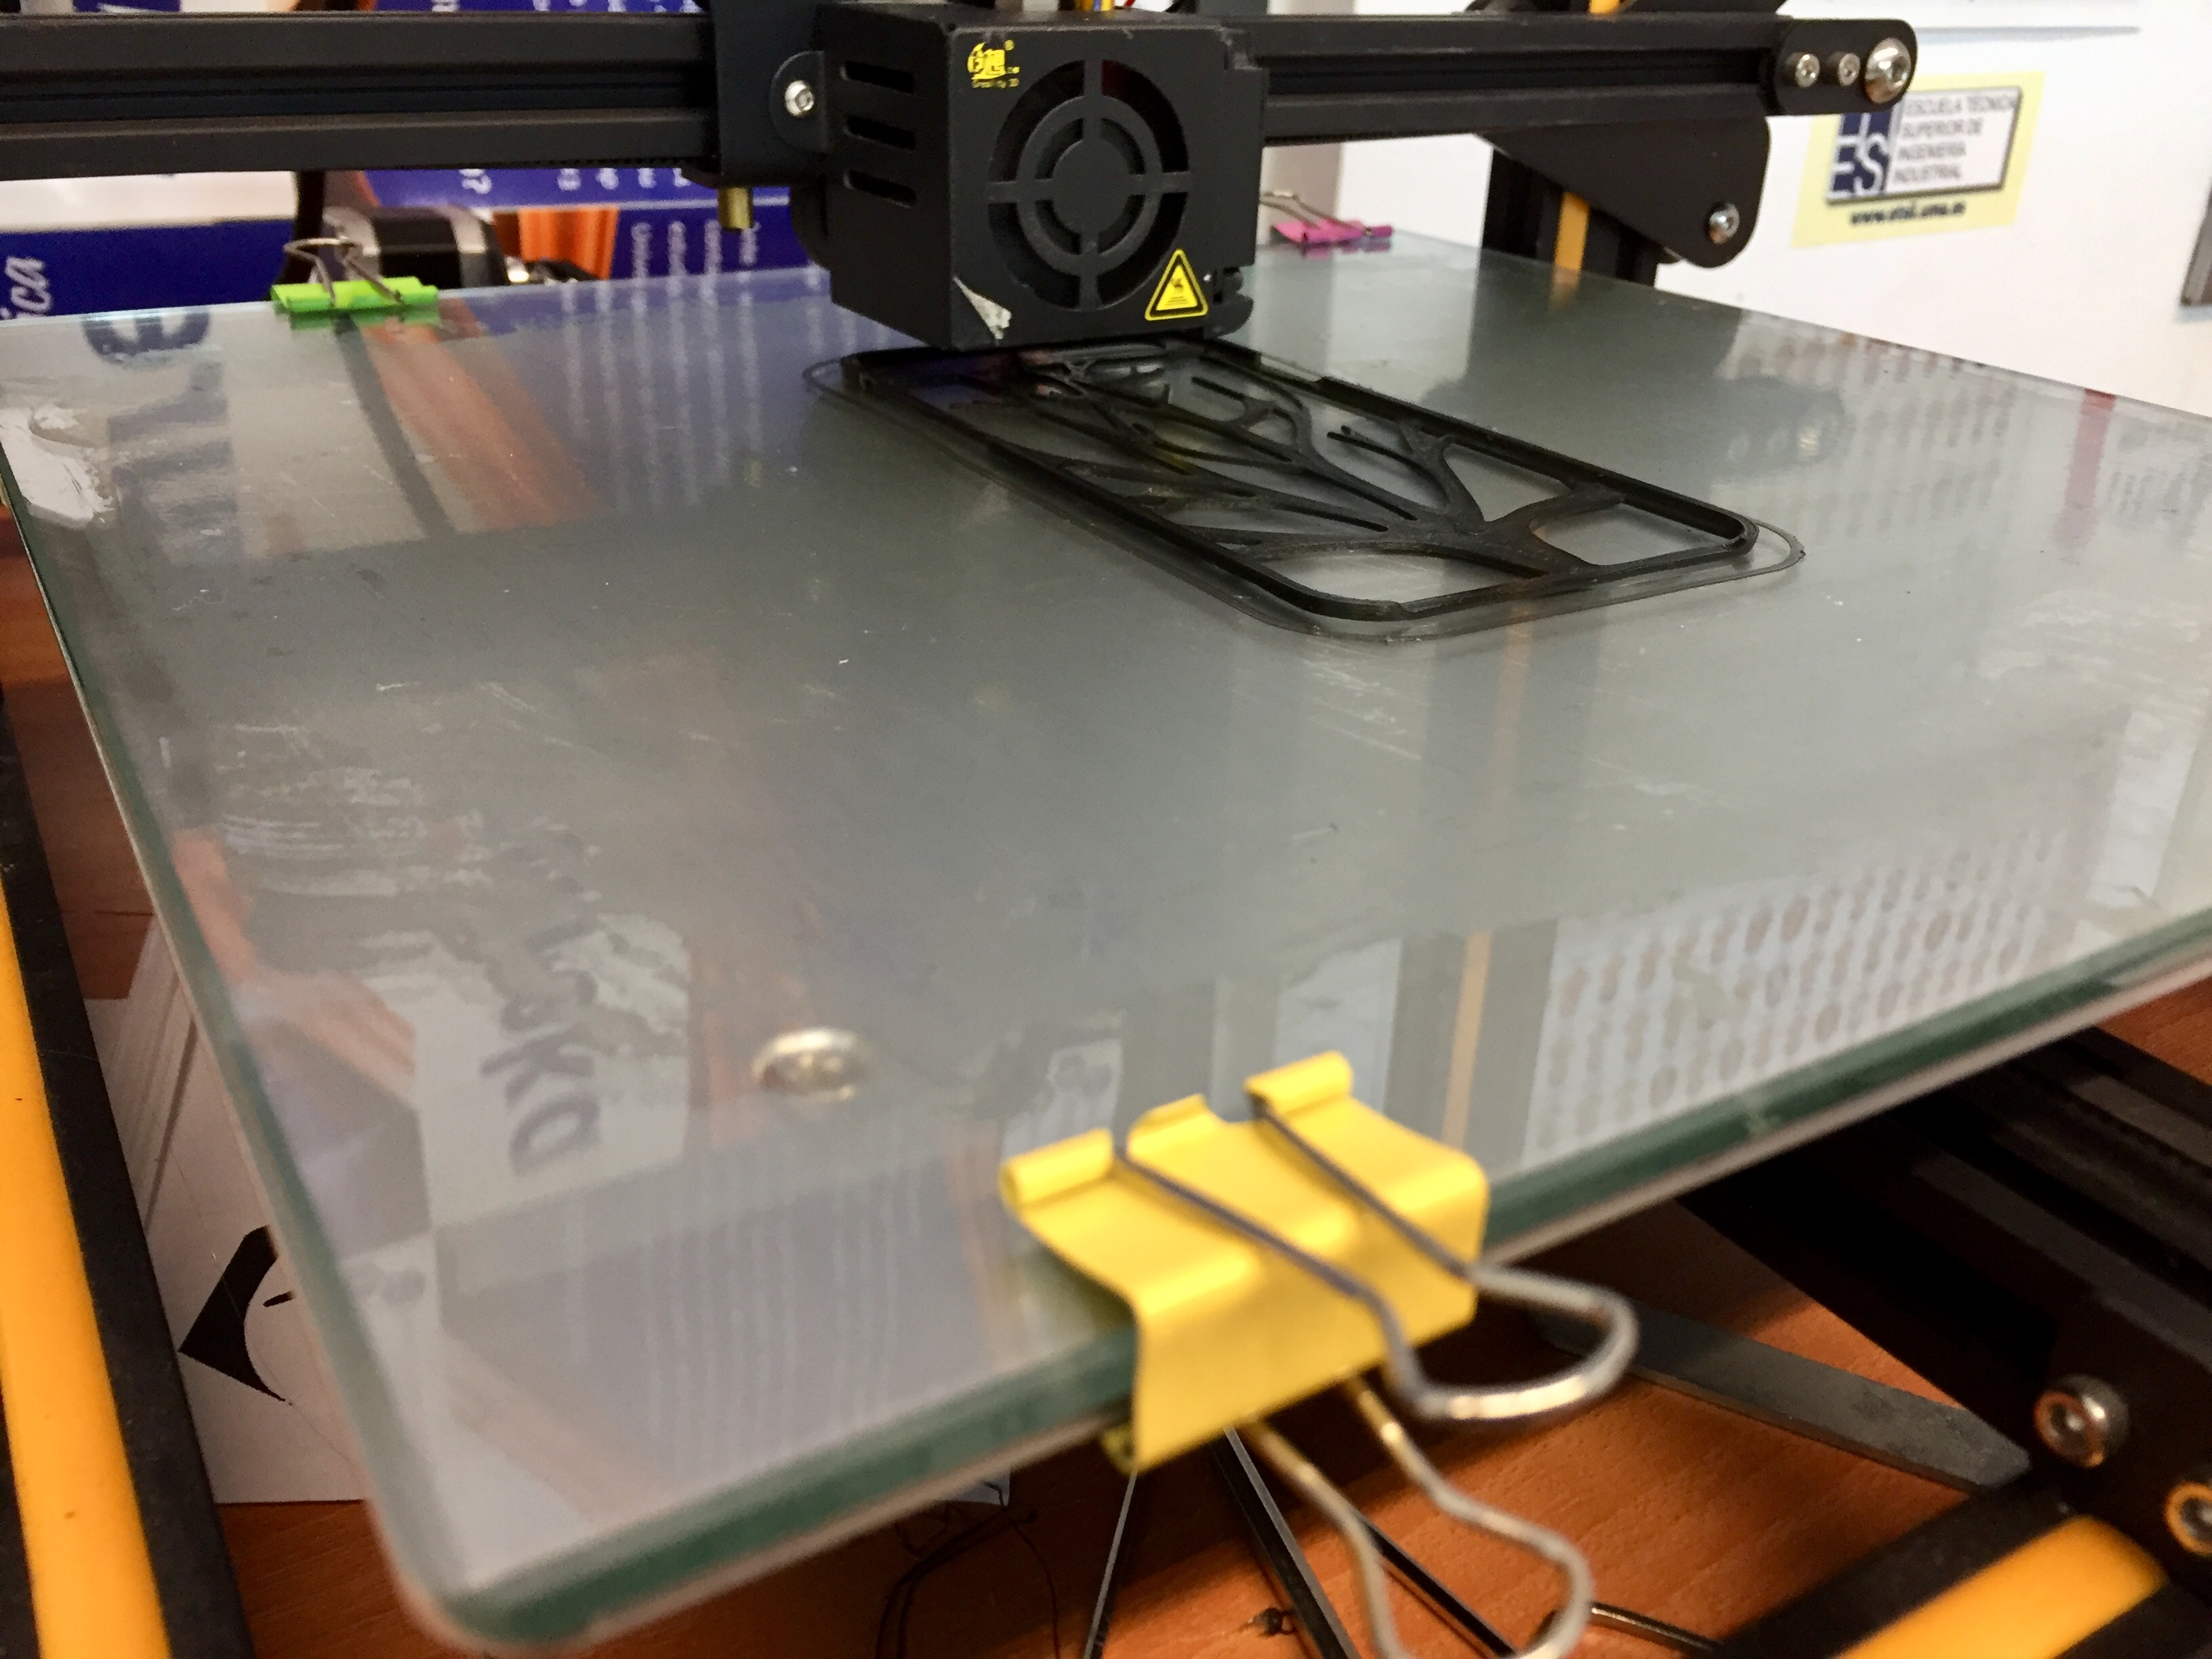
\includegraphics[height=0.8\textheight]{images/cama}
			\caption{Cama de impresión de cristal}
		\end{figure}
	\end{frame}
	\begin{frame}{Finales de carrera}
		\begin{figure}
			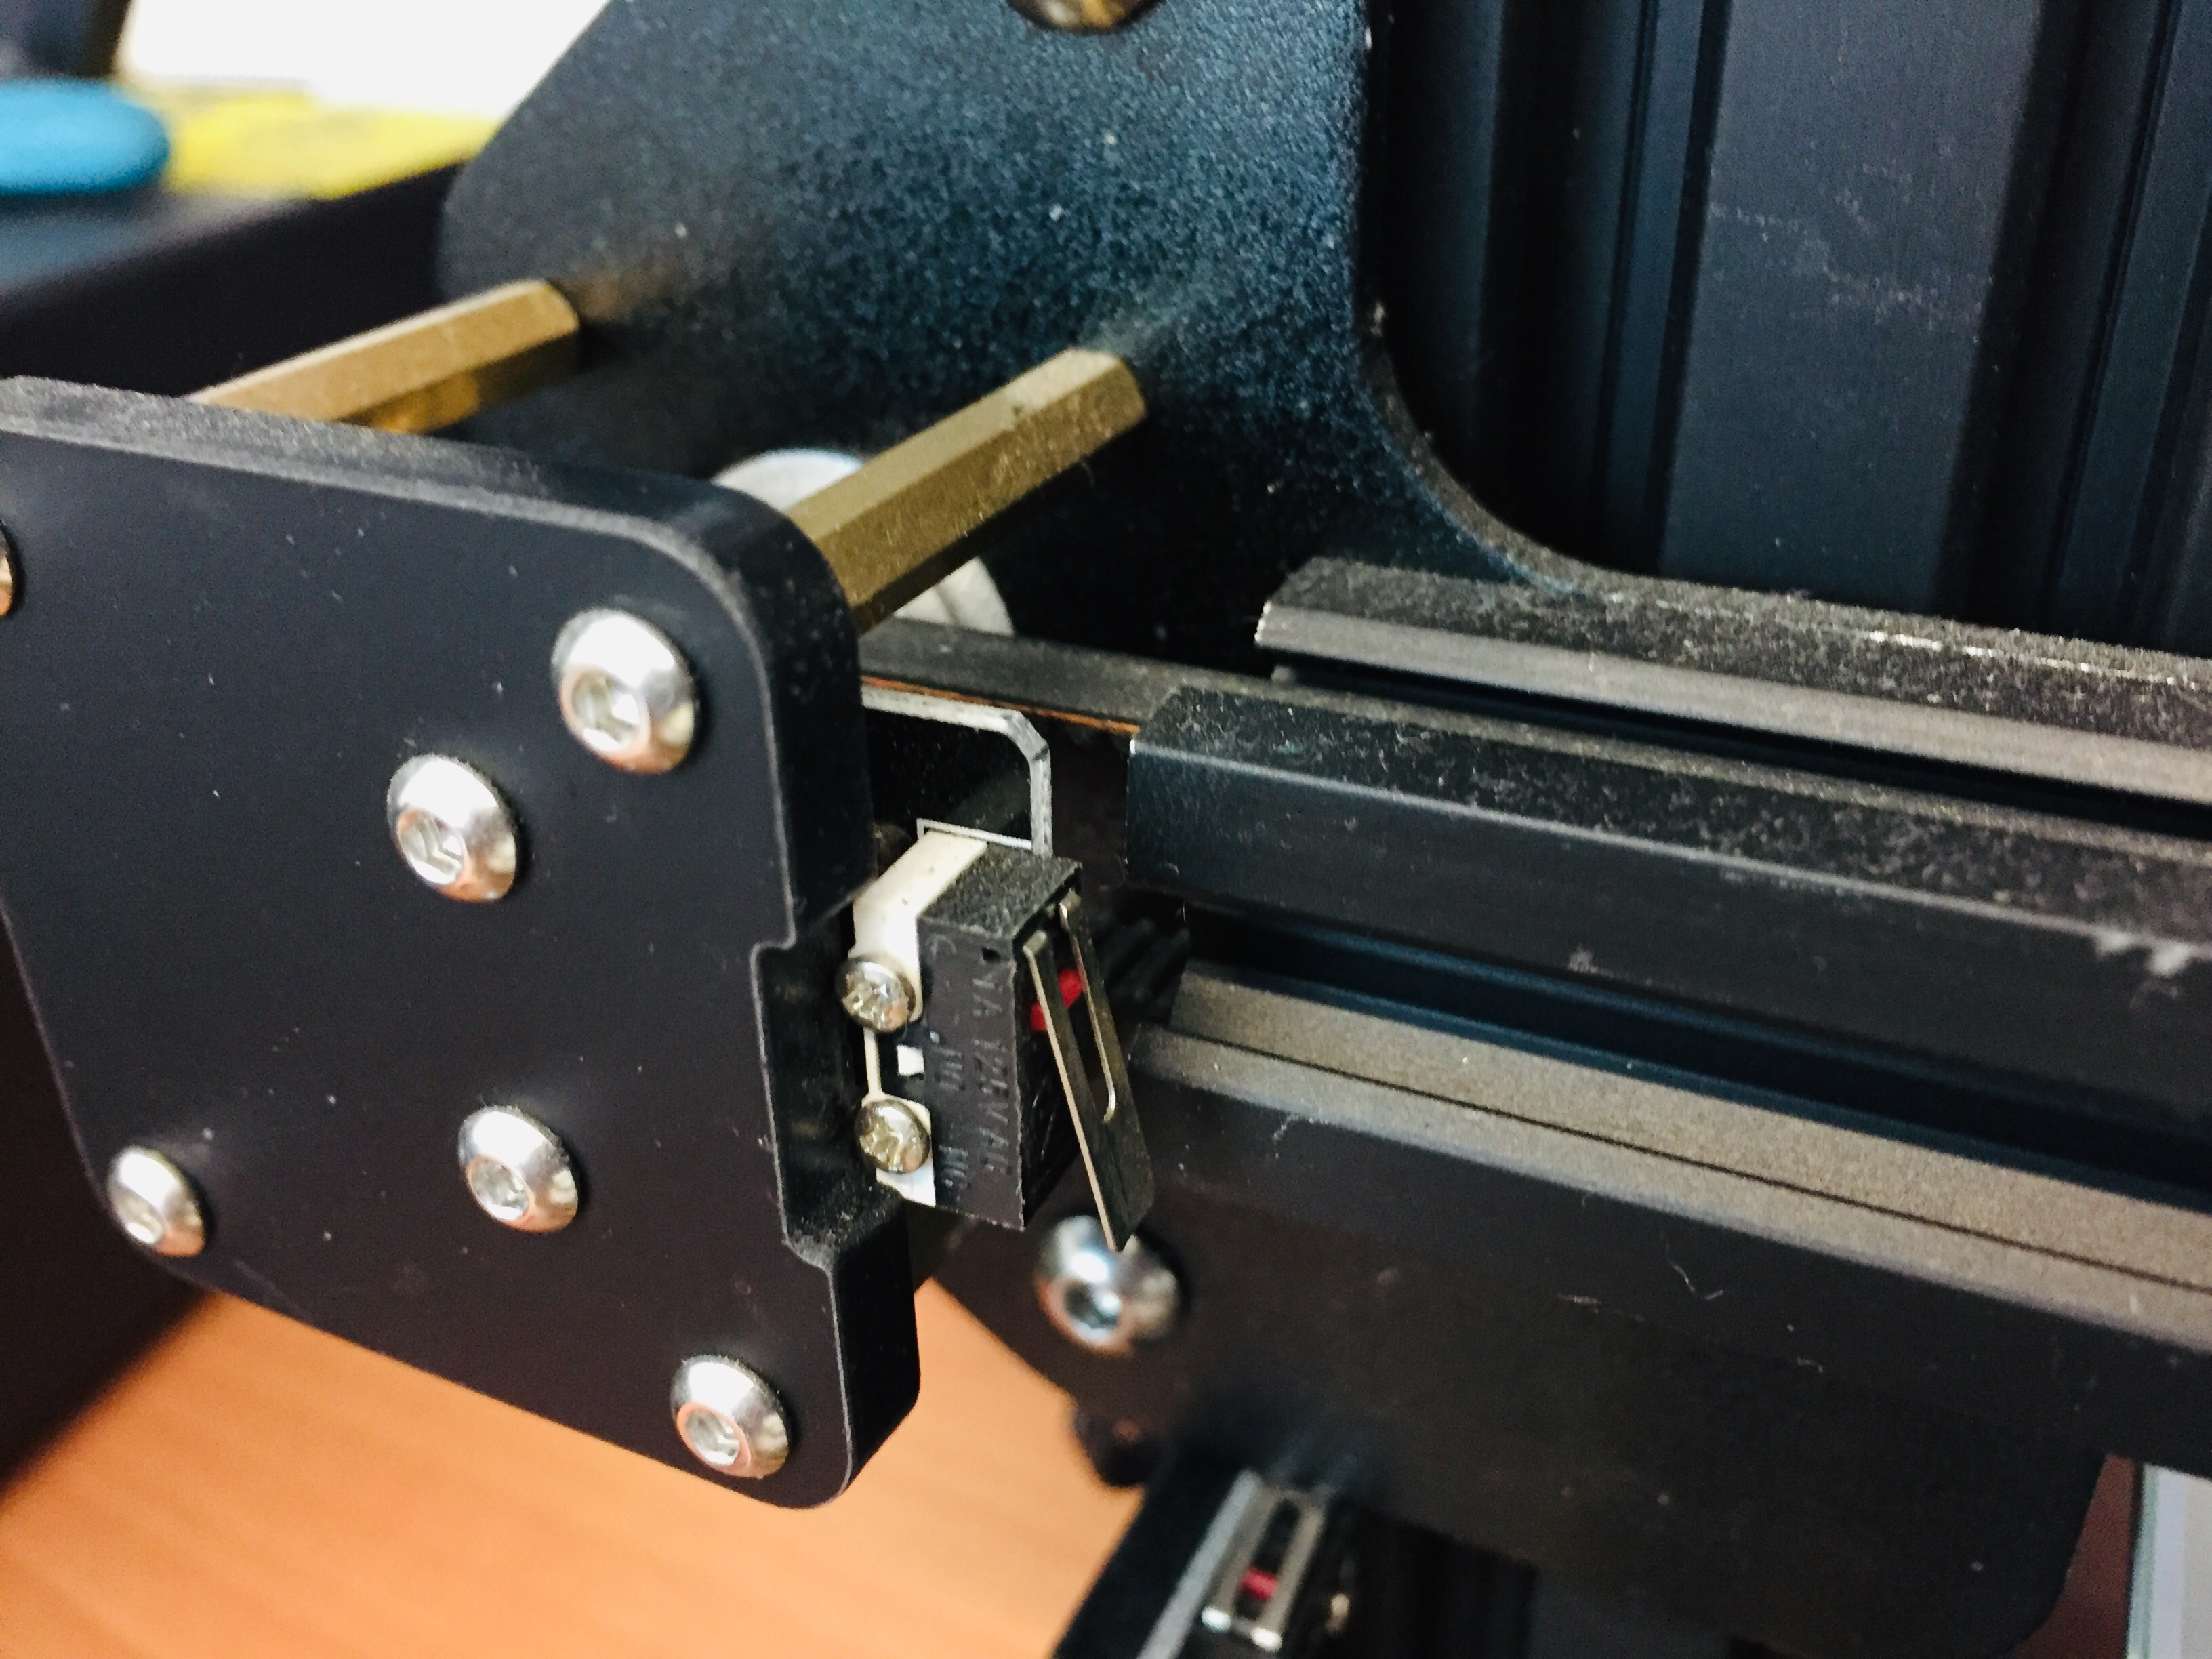
\includegraphics[height=0.8\textheight]{images/final}
			\caption{Final de carrera del eje X}
		\end{figure}
	\end{frame}
	
	\subsection{Materiales}
	\begin{frame}{Ácido Poliláctico (PLA)}
		\begin{columns}[T, onlytextwidth]
			\column{0.5\textwidth}
			Pros
			\begin{itemize}
				\item Bajo coste
				\item Rígido y resistente
				\item Buena precisión dimensional
				\item Larga vida
				\item Biodegradable
			\end{itemize}
			\column{0.5\textwidth}
			Contras
			\begin{itemize}
				\item Poca resistencia al calor
				\item Tiene fallo frágil
				\item No apto para uso en exteriores
			\end{itemize}
		\end{columns}
	\end{frame}
	\begin{frame}{Otros materiales}
		\begin{itemize}
			\item ABS
			\item PETG
			\item TPU
			\item Nylon
			\item \dots
		\end{itemize}
	\end{frame}
	
	\subsection{Modelos}
	\begin{frame}{Dónde conseguir modelos}
		\begin{columns}[T, onlytextwidth]
			\column{0.5\textwidth}
			Diseñarlos en CAD
			\begin{itemize}
				\item Fusion 360
				\item SolidWorks
				\item FreeCAD
			\end{itemize}
			\column{0.5\textwidth}
			Copiarlos
			\begin{itemize}
				\item Thingiverse
				\item GrabCAD
				\item 3D Warehouse
				\item Turbosquid
			\end{itemize}
		\end{columns}
	\end{frame}
	
	\subsection{Slicer}
	\begin{frame}[standout]{Ultimaker-CURA}
		Demostración práctica
	\end{frame}
	
	%%%%%%%%%%%%%%%%%%%%%%%%%%%%%%%%%%%%%%%%
	\section{Antes de imprimir}
	\begin{frame}{Calibración}
		\begin{figure}
			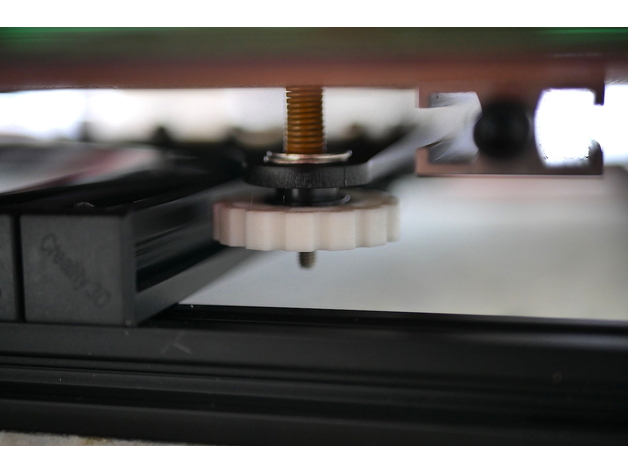
\includegraphics[width=0.75\textwidth]{images/bed_knob}
			\caption{Tuercas de calibración de la cama}
		\end{figure}
	\end{frame}
	\begin{frame}{Cambiar filamento}
		\begin{figure}
			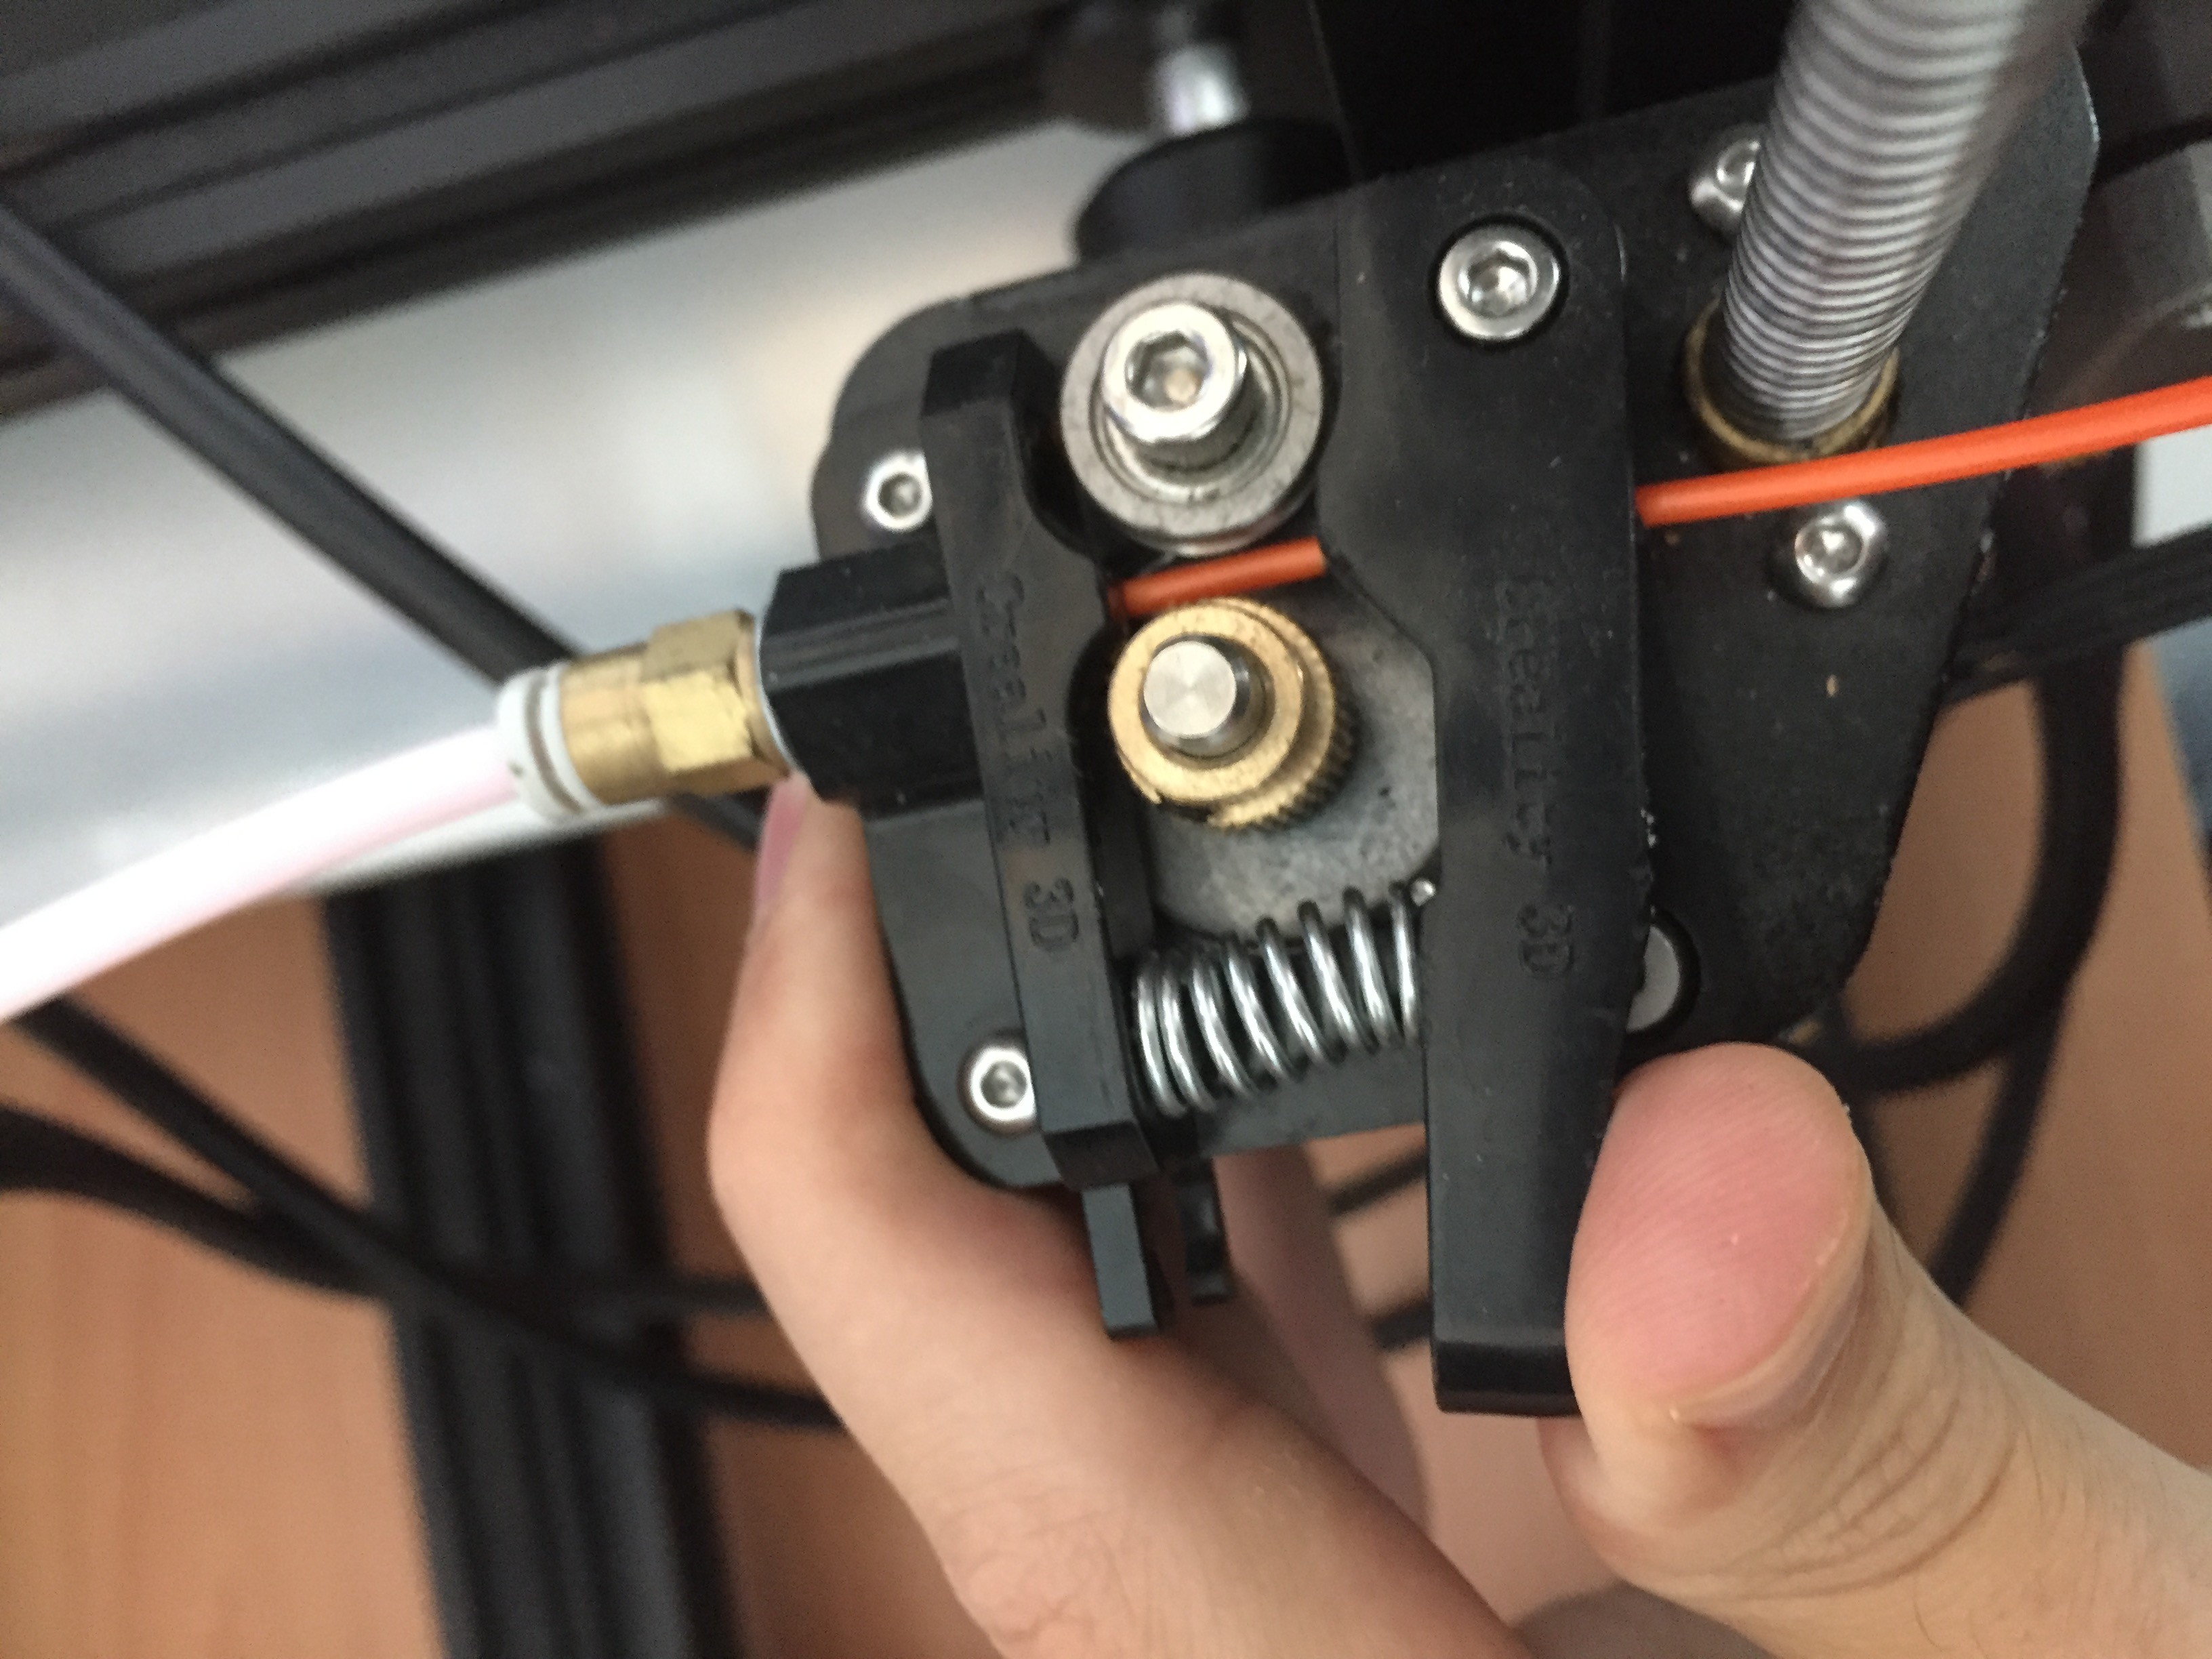
\includegraphics[width=.75\textwidth]{images/cambiar_filamento}
			\caption{Pulsar la palanca para aflojar la presión}
		\end{figure}
	\end{frame}
	\begin{frame}{Adhesivos}
		\begin{figure}
			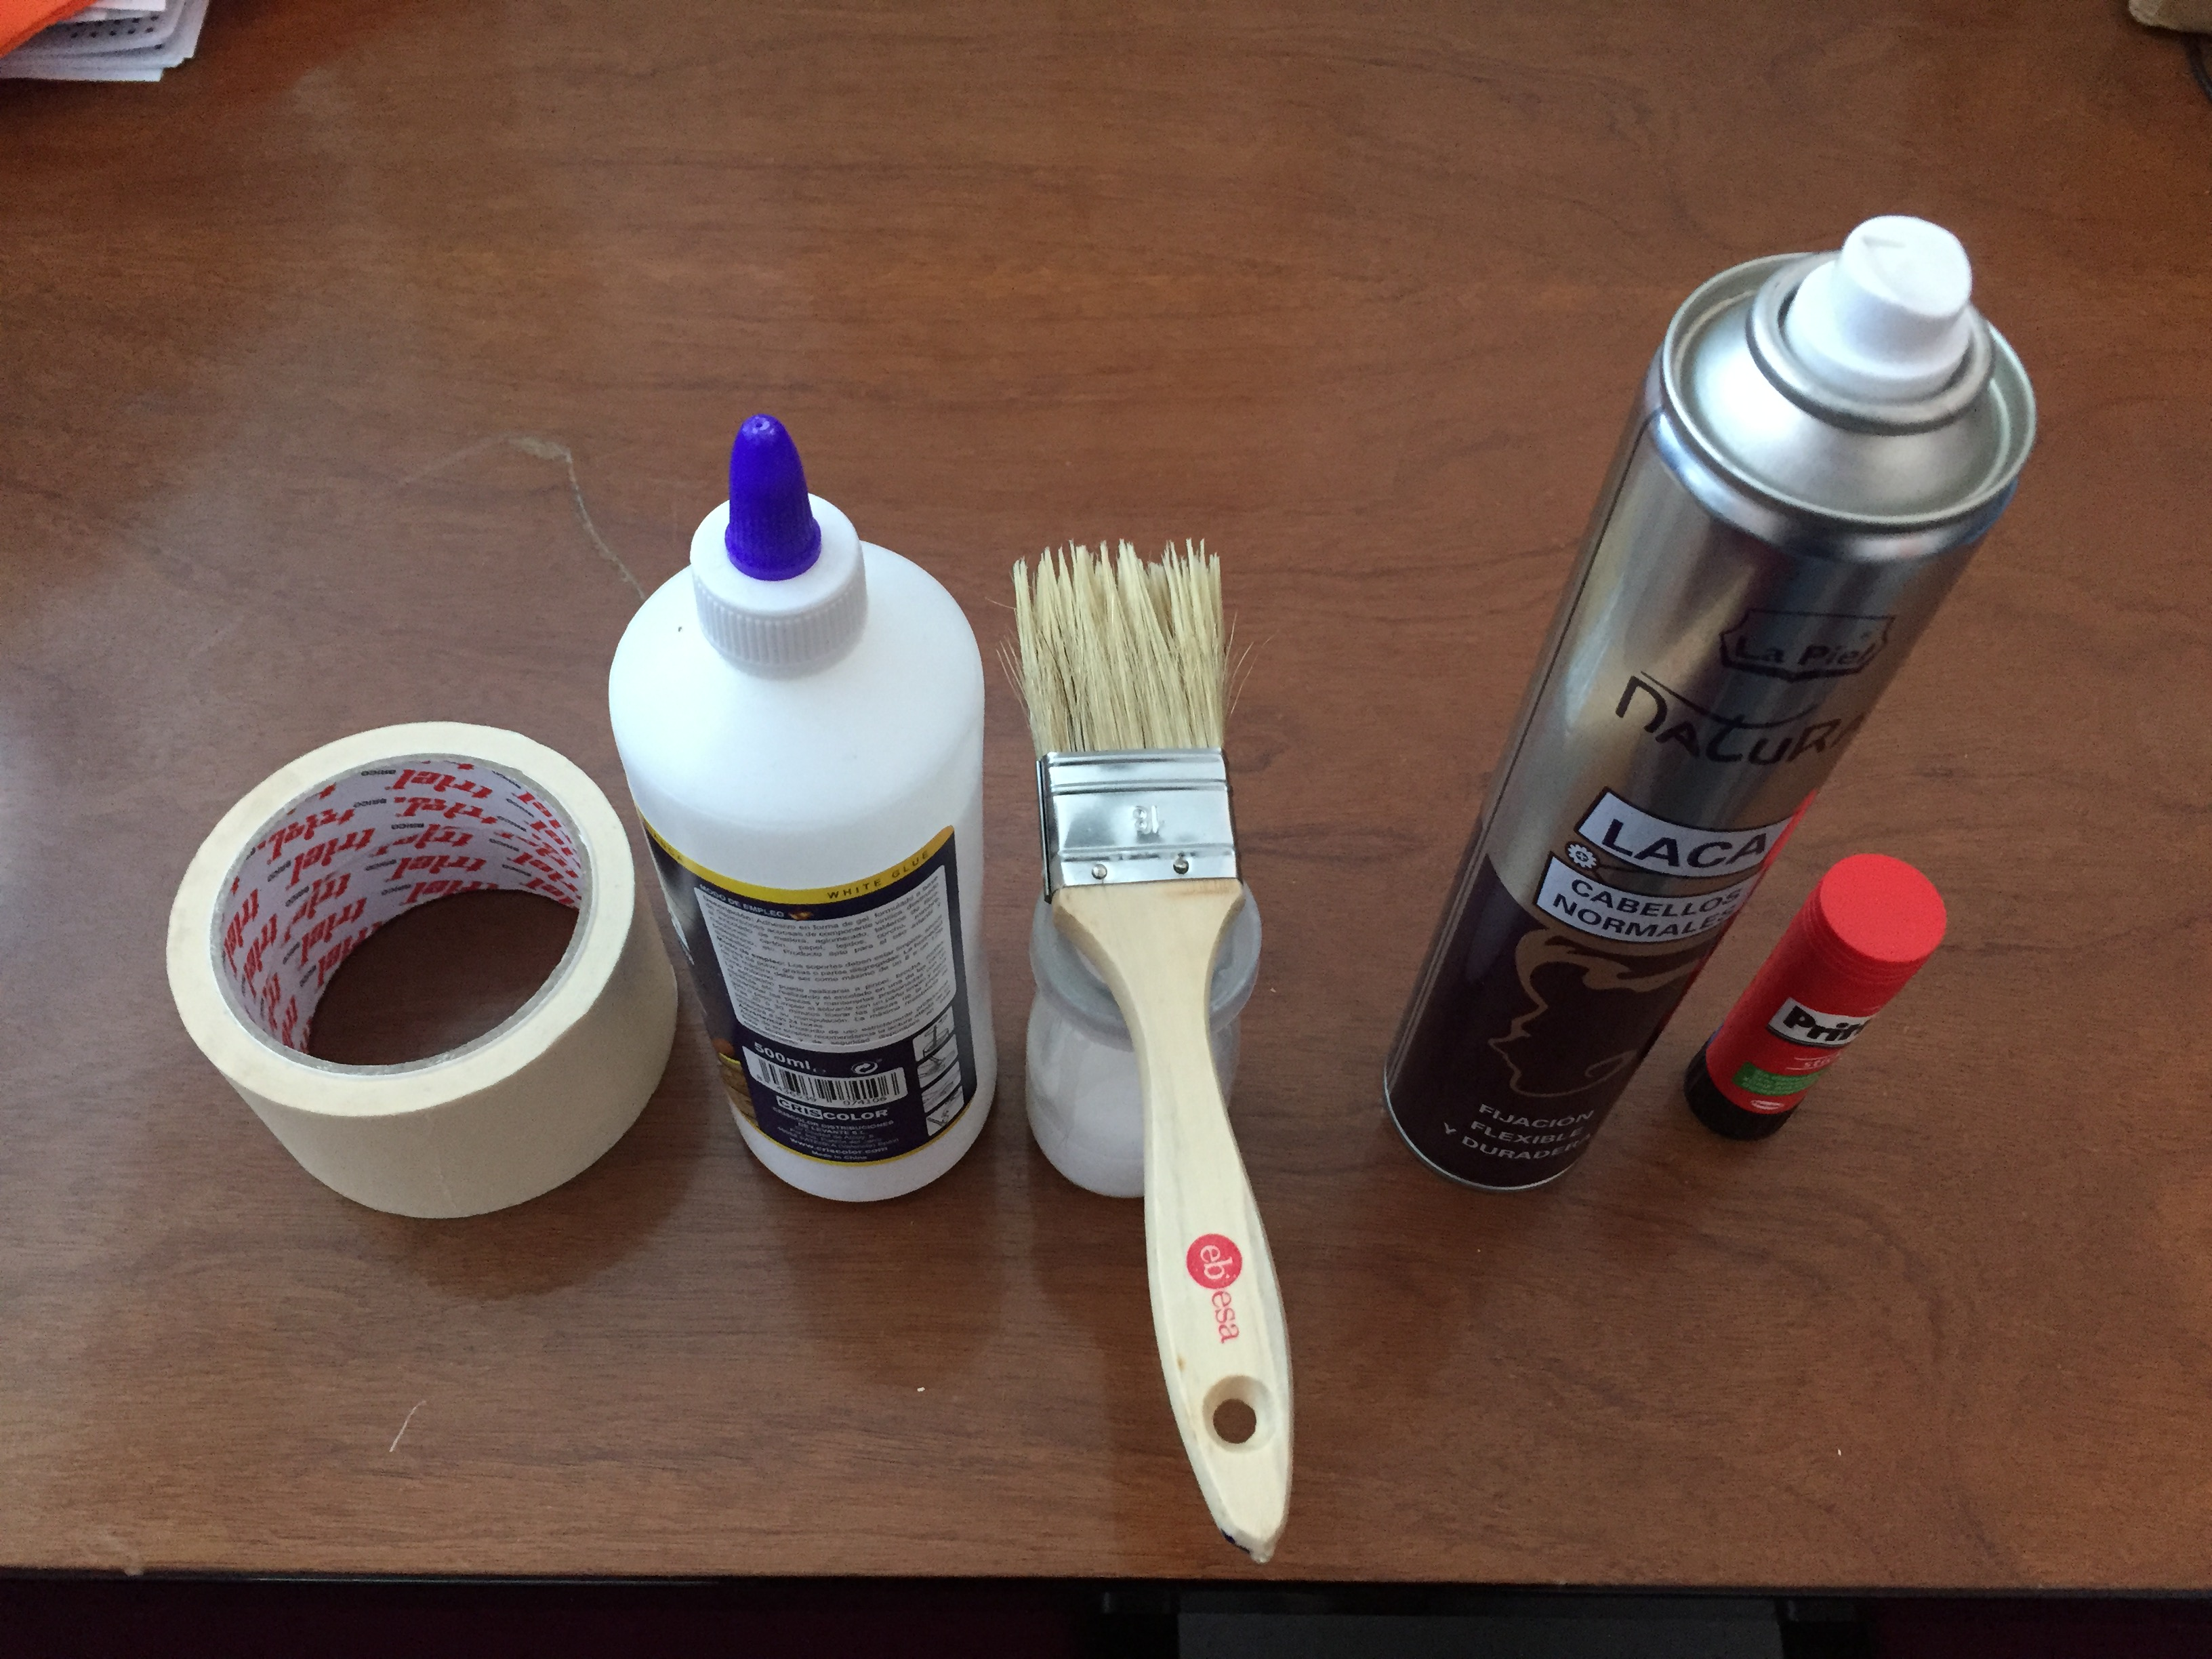
\includegraphics[width=.75\textwidth]{images/adhesivos}
			\caption{Distintos adhesivos ofrecen distintos resultados}
		\end{figure}
	\end{frame}
	
	%%%%%%%%%%%%%%%%%%%%%%%%%%%%%%%%%%%%%%%%
	\section{Durante la impresión}
	\begin{frame}{Primera capa}
		\begin{figure}
			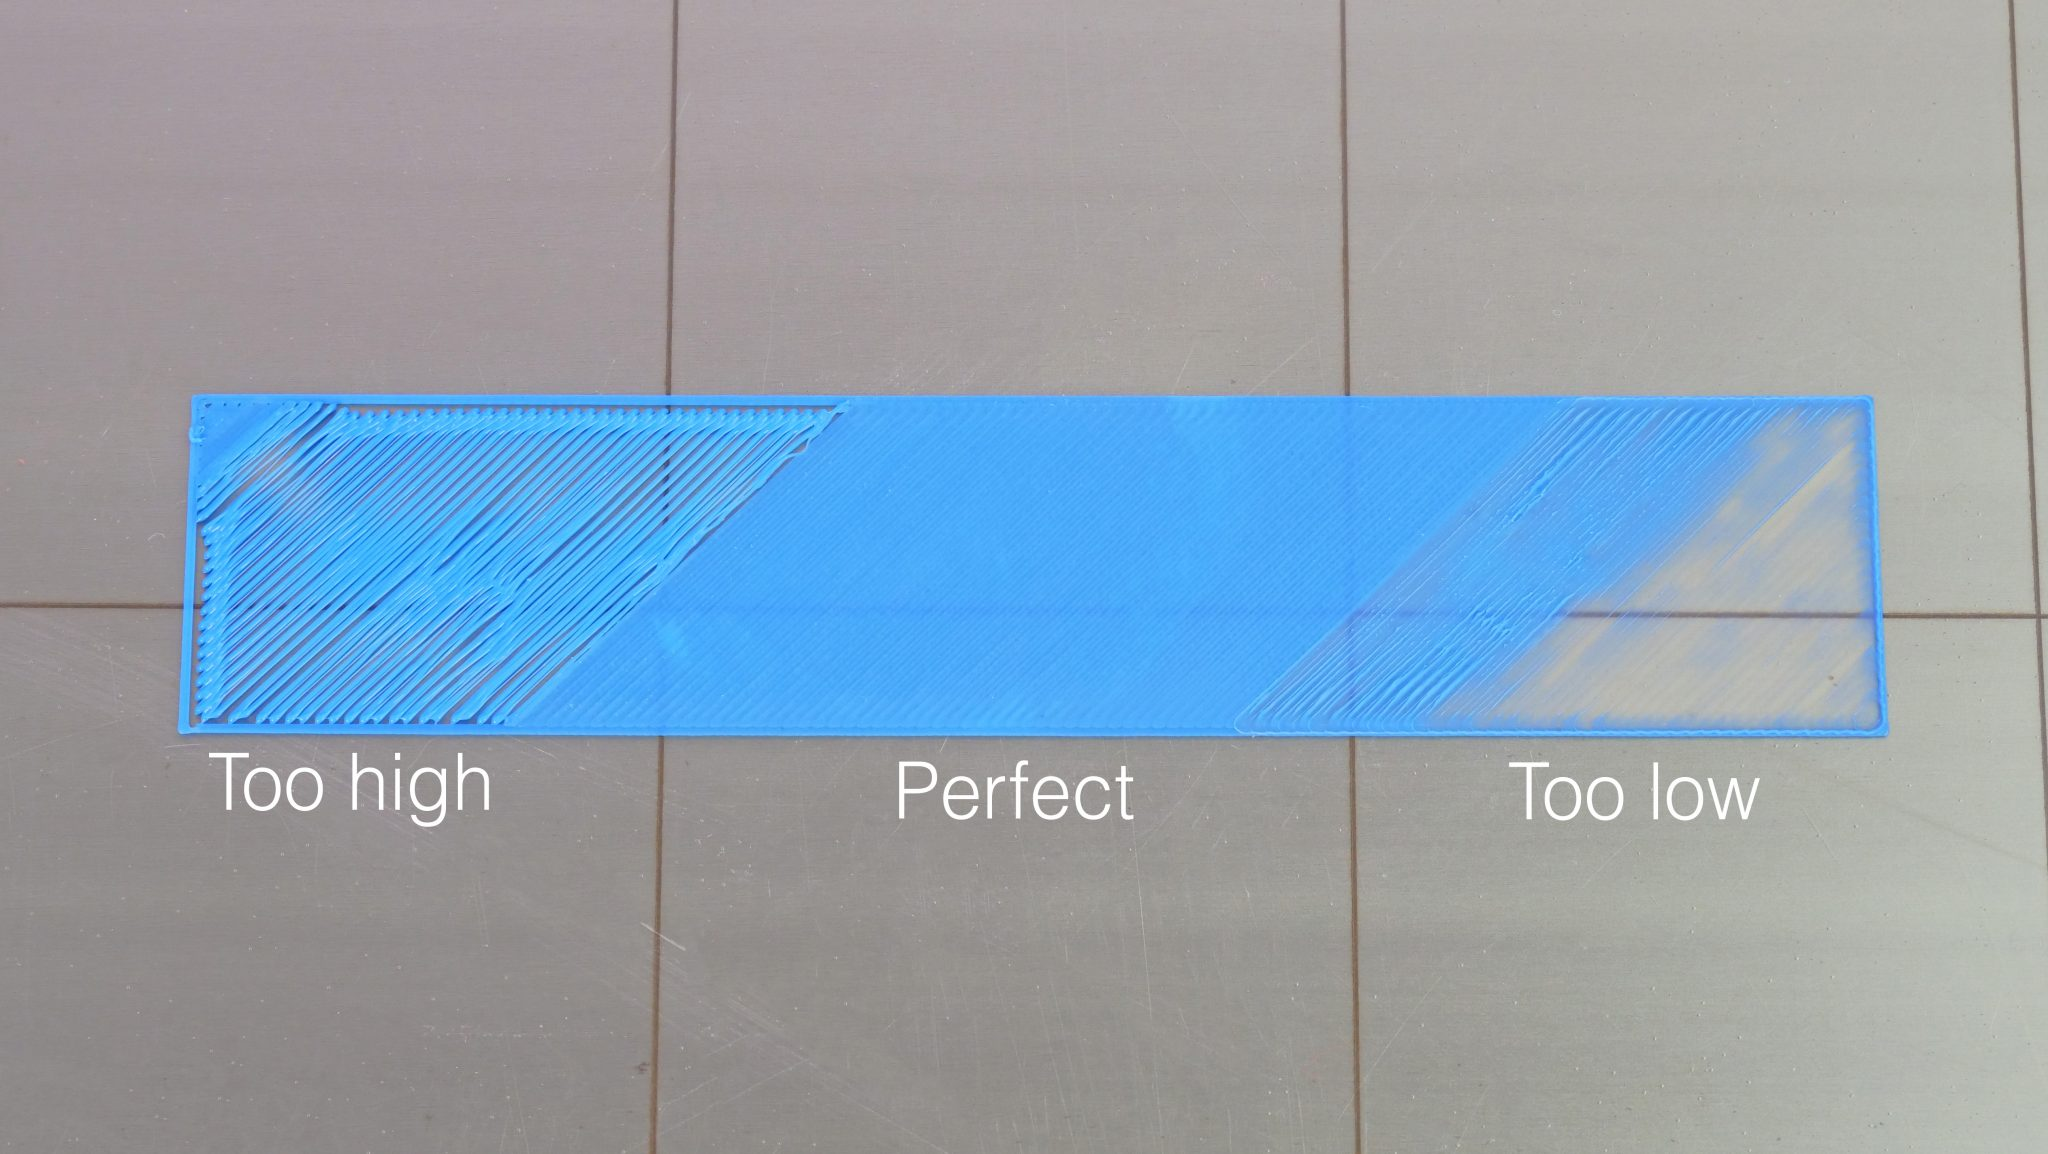
\includegraphics[width=\textwidth]{images/first_layer}
			\caption{La altura de la primera capa es crítica}
		\end{figure}
	\end{frame}
	\begin{frame}{Problemas comunes}
		\begin{columns}
			\column{0.5\textwidth}
				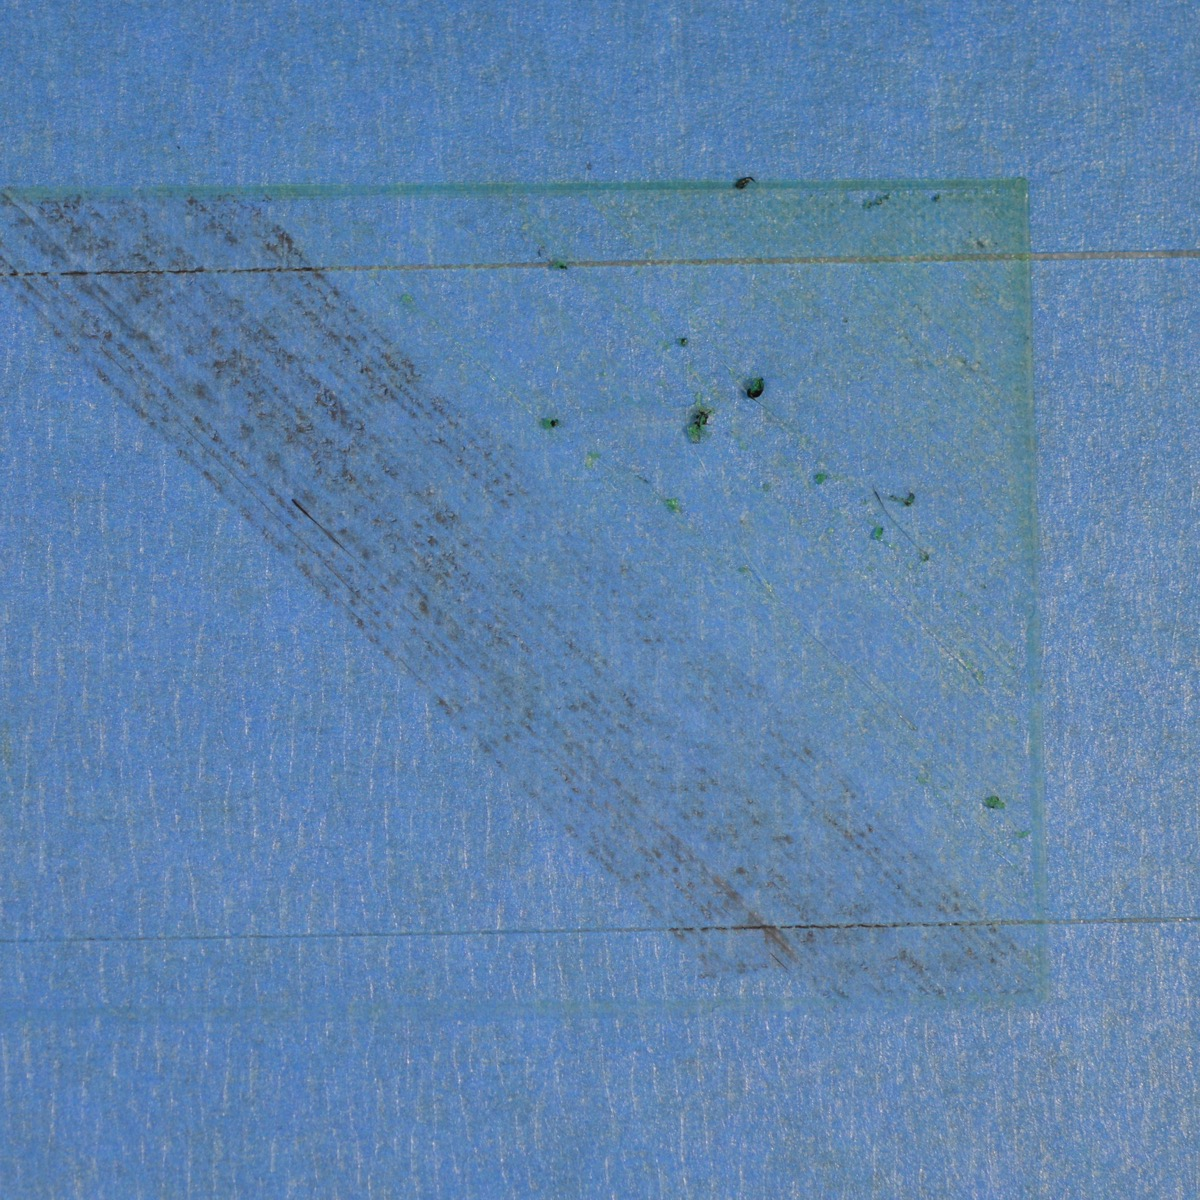
\includegraphics[width=\textwidth]{images/Not-Extruding-At-Start}
			\column{0.5\textwidth}
				\textbf{No hay extrusión al comienzo}
				\begin{itemize}
					\item No hay plástico
					\item Boquilla muy próxima a la cama
					\item La rueda del extrusor ha limado el filamento
					\item Hay un atoramiento
				\end{itemize}
		\end{columns}
	\end{frame}
	\begin{frame}{Problemas comunes}
		\begin{columns}
			\column{0.5\textwidth}
				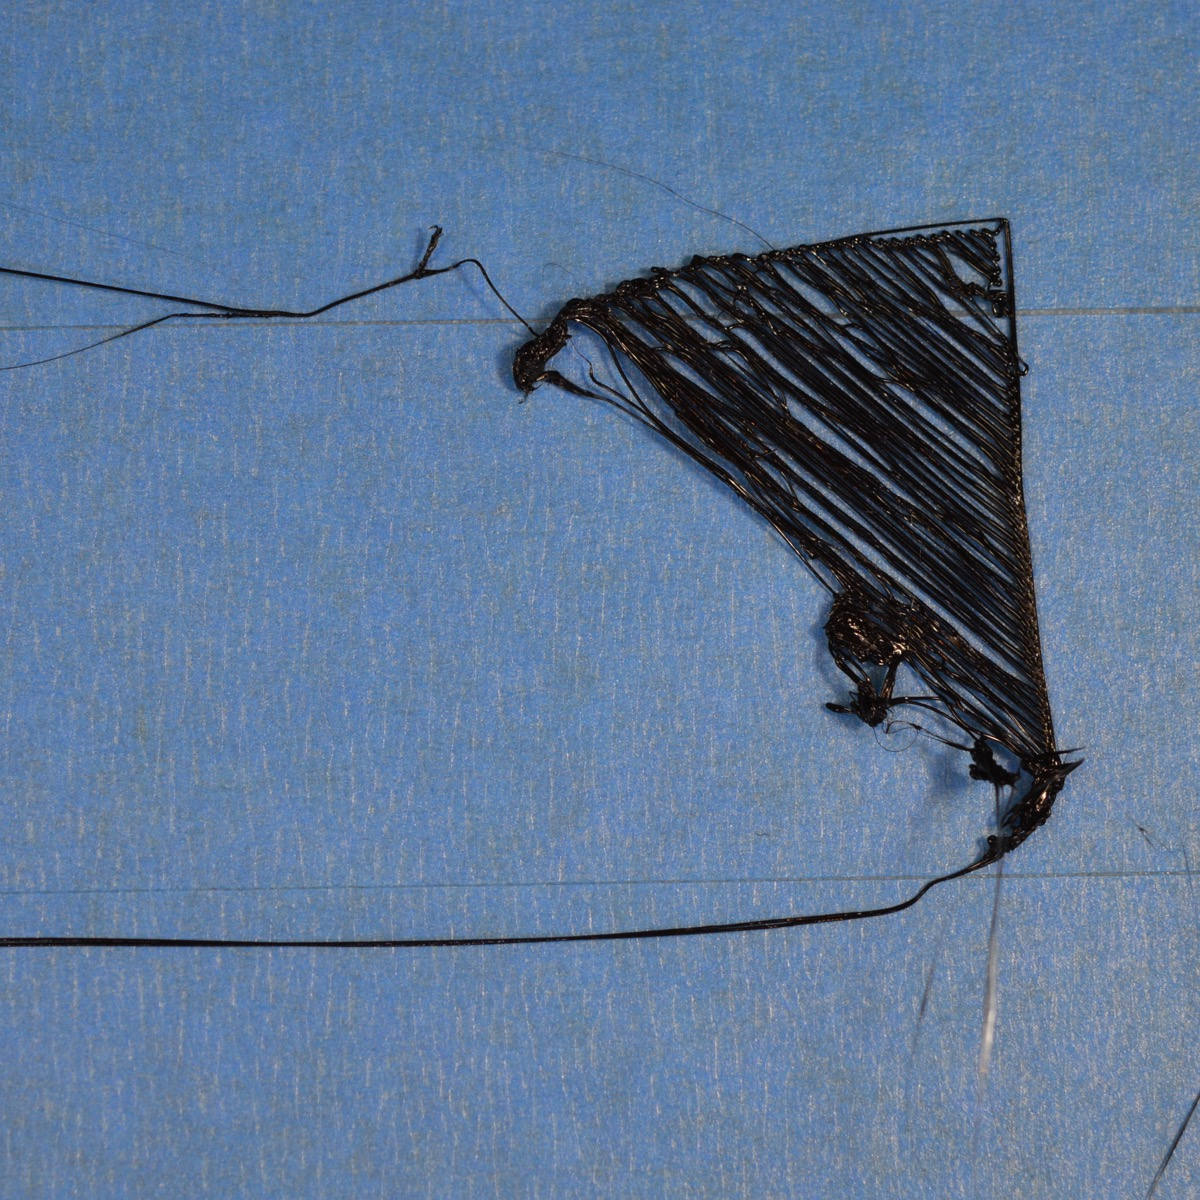
\includegraphics[width=\textwidth]{images/Print-Not-Sticking-To-Bed}
			\column{0.5\textwidth}
				\textbf{La pieza no se adhiere a la cama}
				\begin{itemize}
					\item La cama no está nivelada
					\item La boquilla está muy alejada
					\item La velocidad de la primera capa es muy alta
					\item Ajustes de temperatura
					\item Fallo en el adhesivo
					\item Cuando todo falla: borde o balsa
				\end{itemize}
		\end{columns}
	\end{frame}
	\begin{frame}{Problemas comunes}
		\begin{columns}
			\column{0.5\textwidth}
				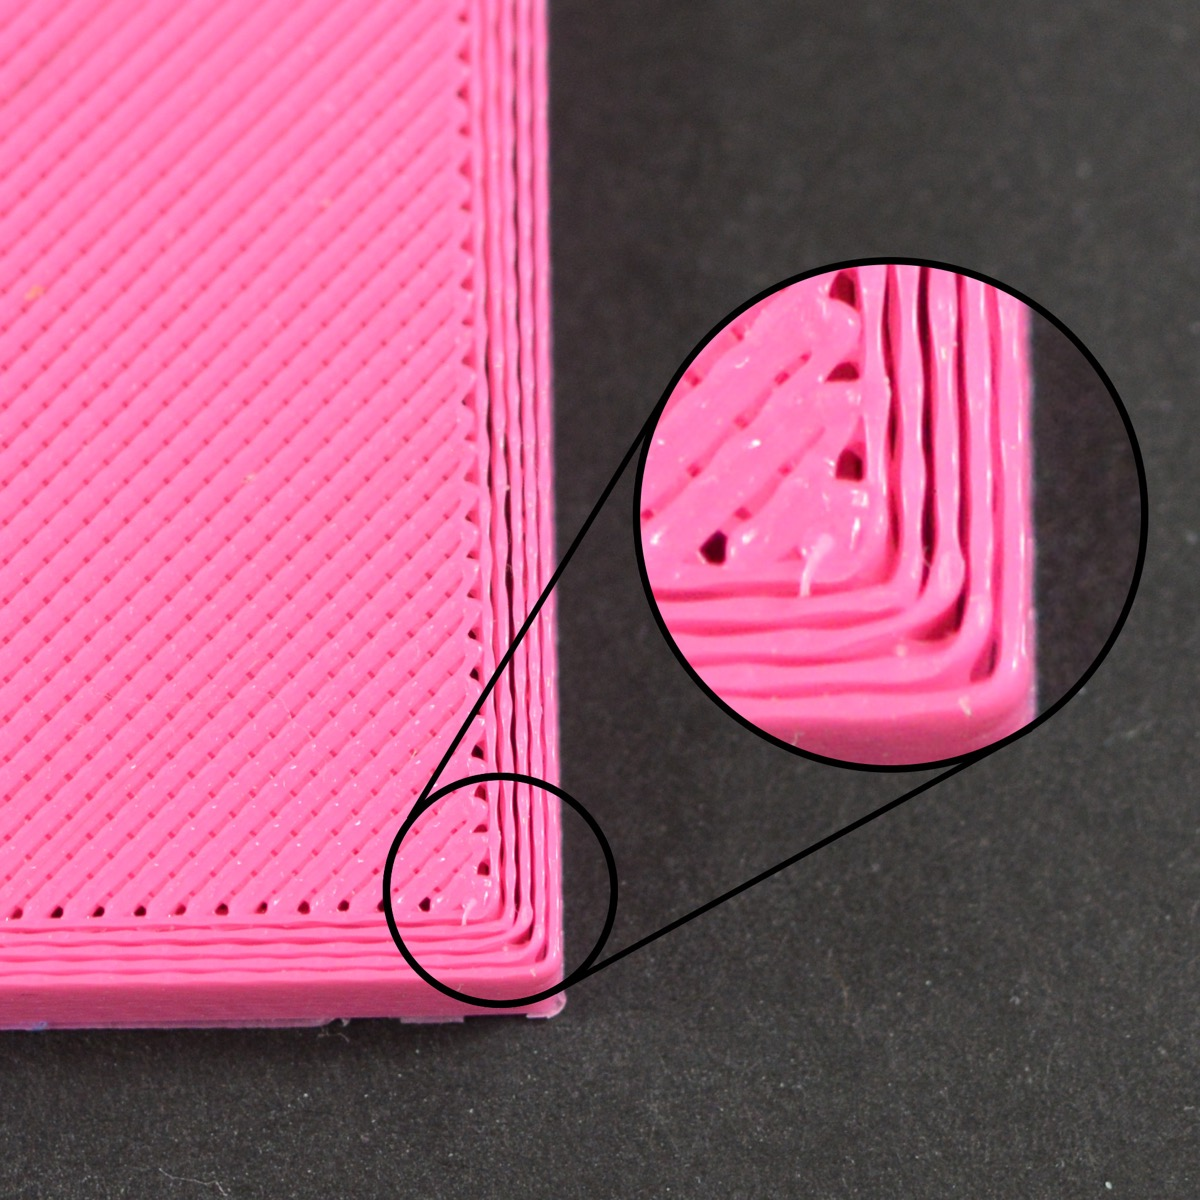
\includegraphics[width=\textwidth]{images/Under-Extruding}
			\column{0.5\textwidth}
				\textbf{Infraextrusión}
				\begin{itemize}
					\item Multiplicador de extrusión
				\end{itemize}
		\end{columns}
	\end{frame}
	\begin{frame}{Problemas comunes}
		\begin{columns}
			\column{0.5\textwidth}
				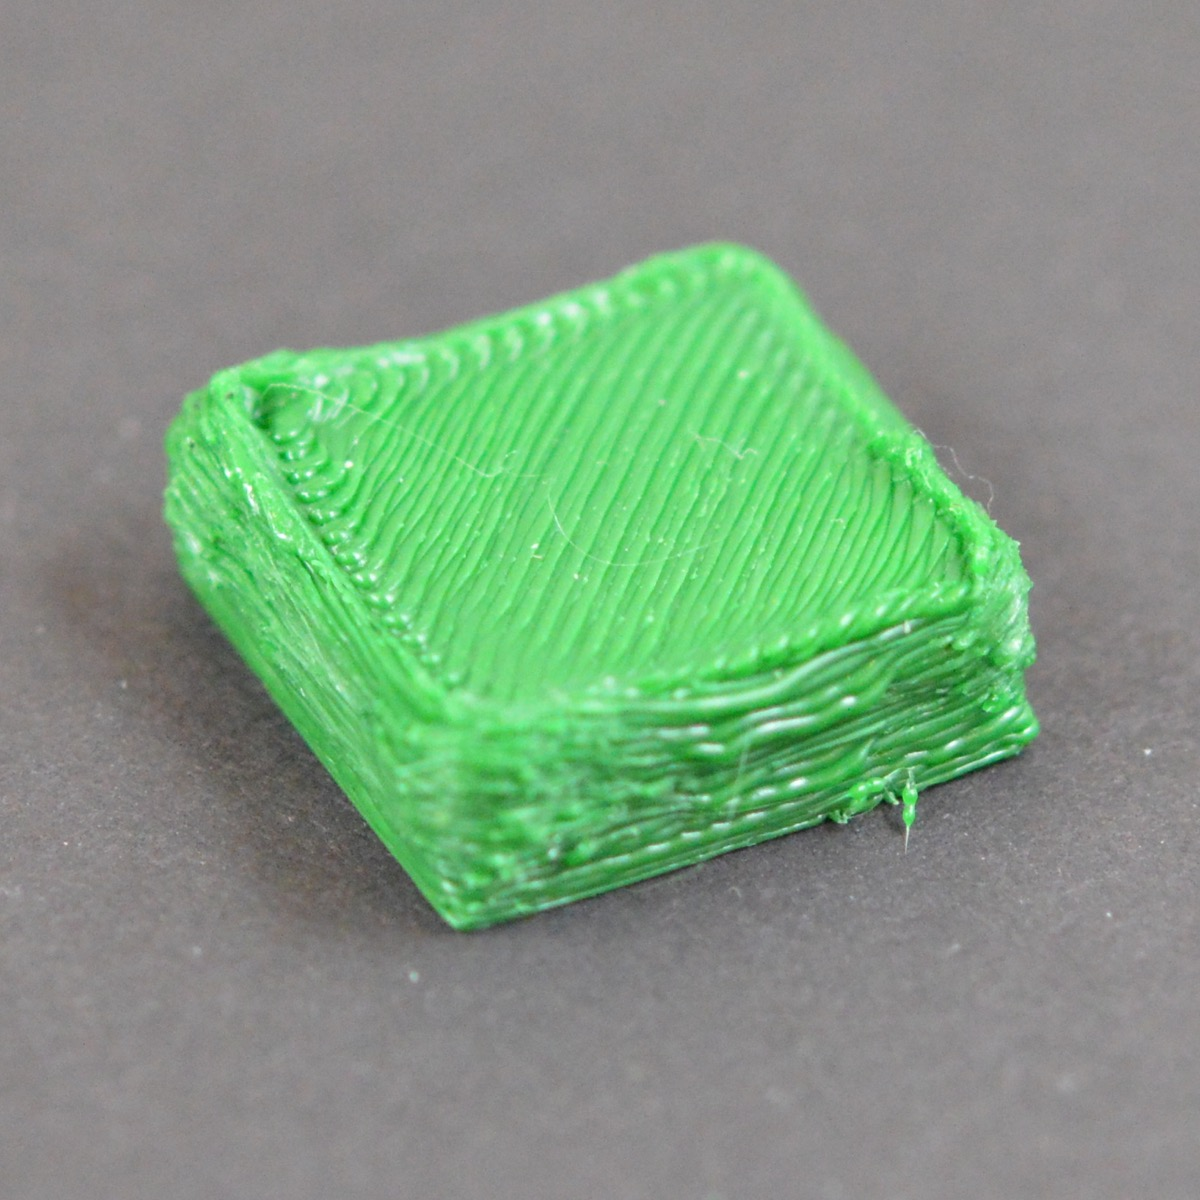
\includegraphics[width=\textwidth]{images/Over-Extruding}
			\column{0.5\textwidth}
				\textbf{Sobreextrusión}
				\begin{itemize}
					\item Multiplicador de extrusión
				\end{itemize}
		\end{columns}
	\end{frame}
	\begin{frame}{Problemas comunes}
		\begin{columns}
			\column{0.5\textwidth}
				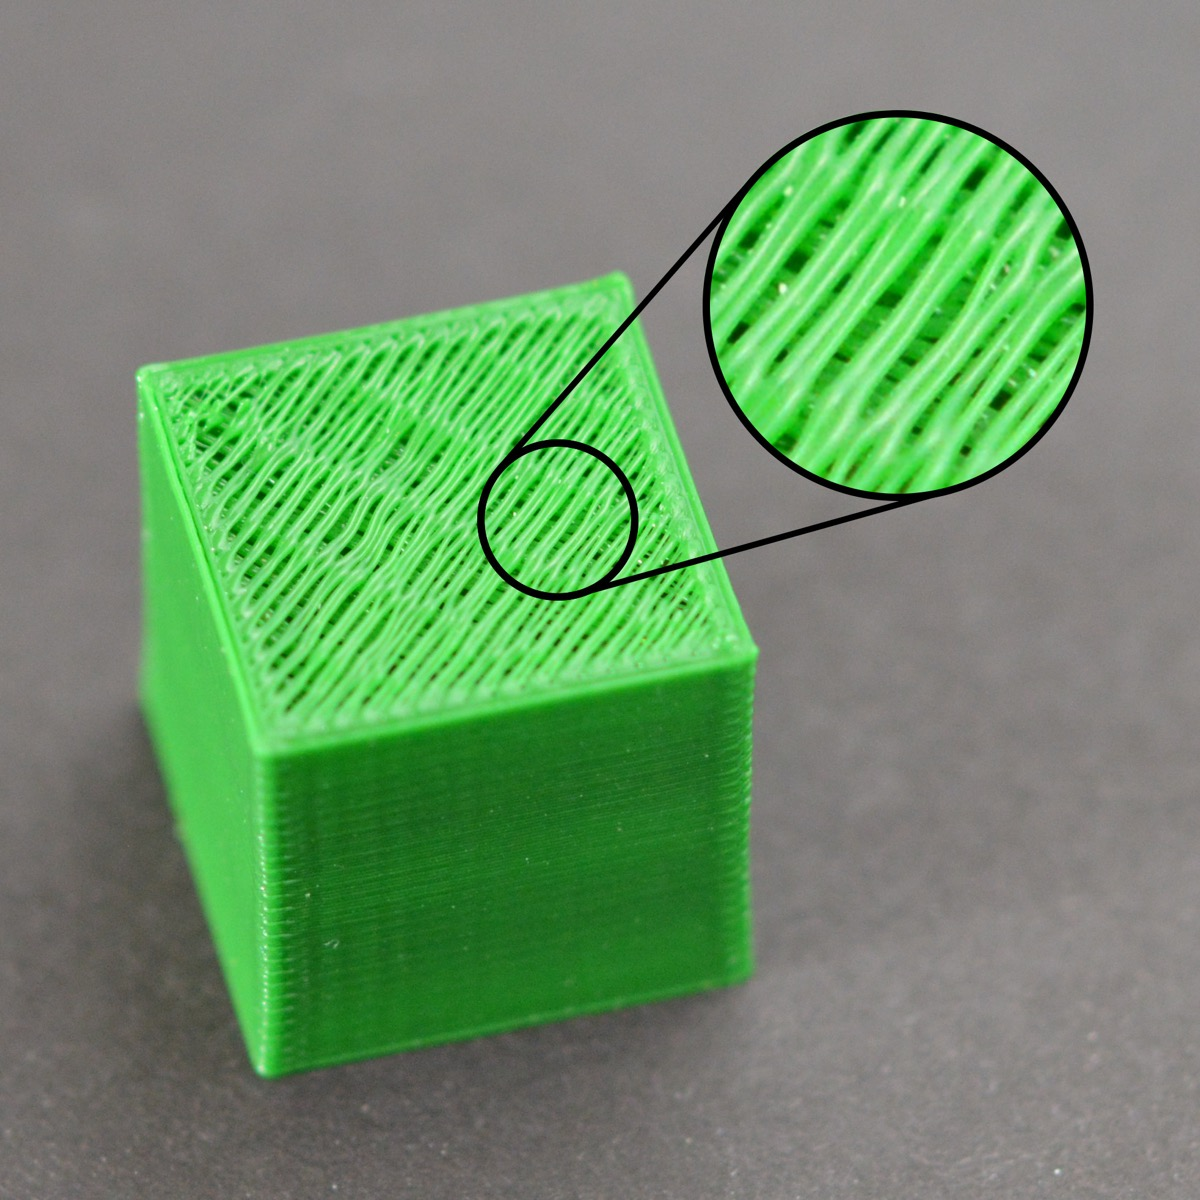
\includegraphics[width=\textwidth]{images/Holes-Or-Gaps-In-Top-Layers}
			\column{0.5\textwidth}
				\textbf{Huecos en las capas superiores}
				\begin{itemize}
					\item Insuficiente número de capas superiores
					\item Porcentaje de relleno demasiado bajo
					\item Infraextrusión
				\end{itemize}
		\end{columns}
	\end{frame}
	\begin{frame}{Problemas comunes}
		\begin{columns}
			\column{0.5\textwidth}
				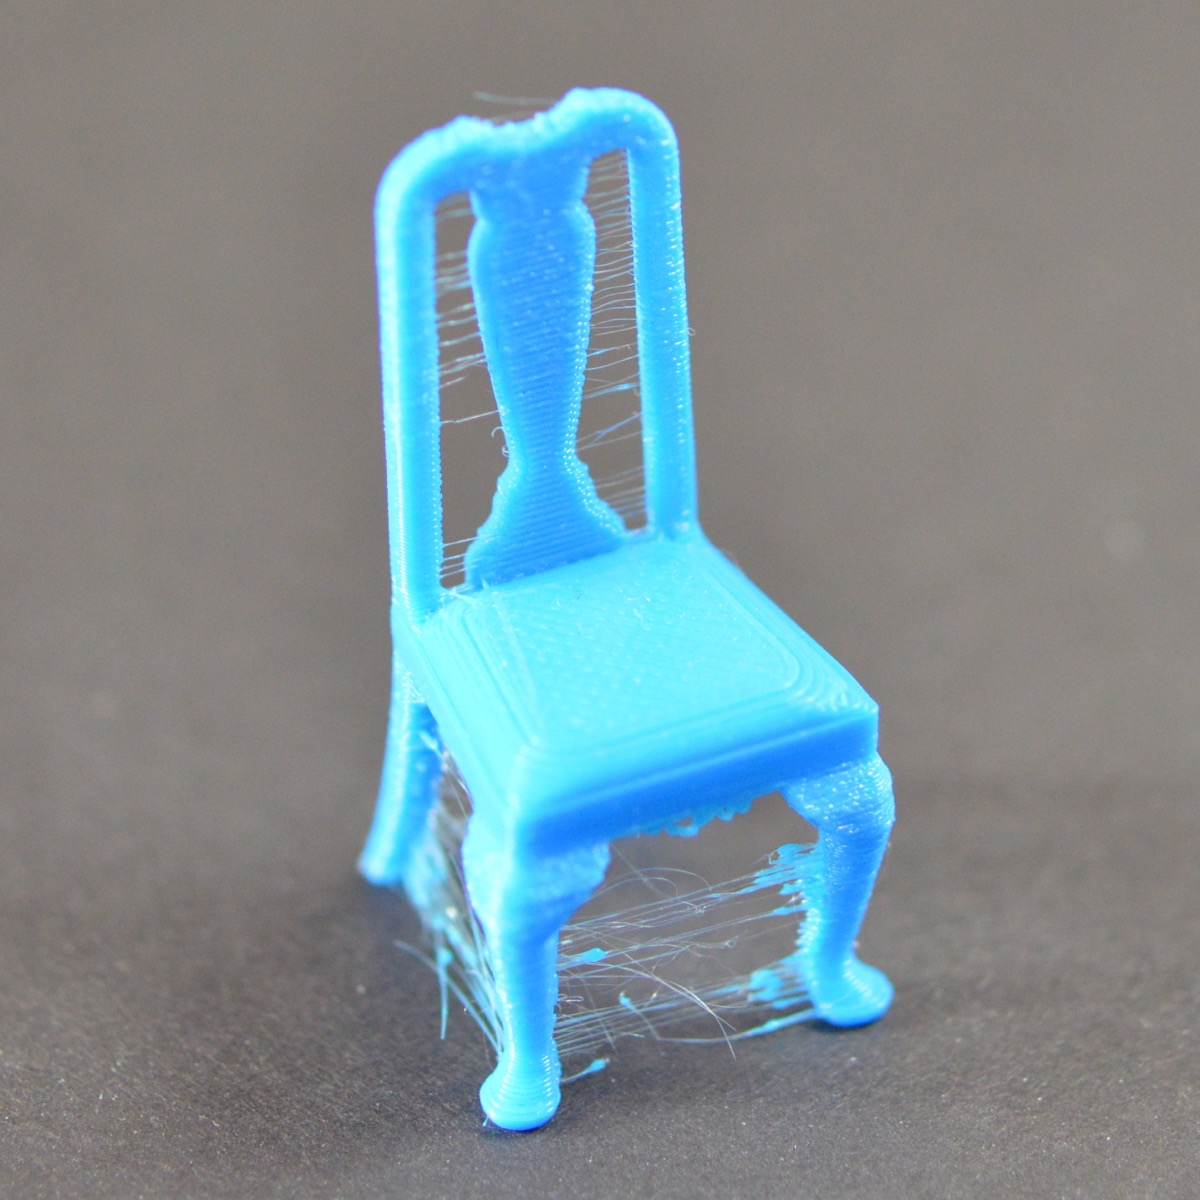
\includegraphics[width=\textwidth]{images/Hairs-And-Stringing}
			\column{0.5\textwidth}
				\textbf{``Hilos'' en la pieza}
				\begin{itemize}
					\item Distancia de retracción
					\item Velocidad de retracción
					\item Temperatura muy elevada
					\item Distancias de viaje muy largas
					\item Velocidad de viaje
				\end{itemize}
		\end{columns}
	\end{frame}
	\begin{frame}{Problemas comunes}
		\begin{columns}
			\column{0.5\textwidth}
				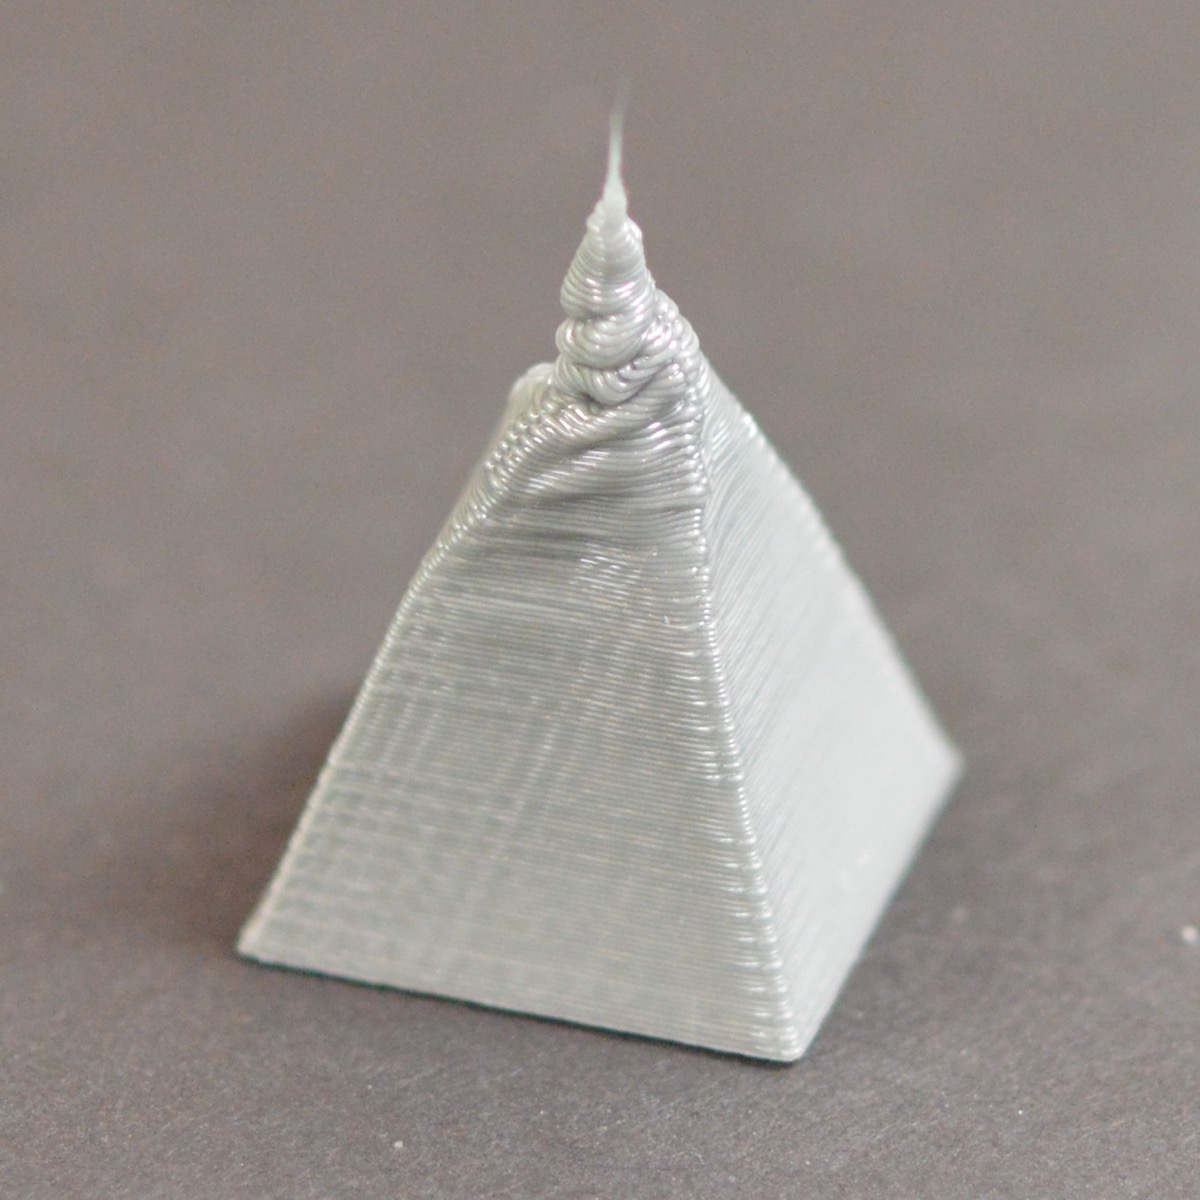
\includegraphics[width=\textwidth]{images/Over-Heating}
			\column{0.5\textwidth}
				\textbf{Sobrecalentamiento}
				\begin{itemize}
					\item Refrigeración insuficiente
					\item Temperatura de impresión demasiado alta
					\item Velocidad demasiado alta
					\item Cuando todo falla: Imprimir piezas de forma individual
				\end{itemize}
		\end{columns}
	\end{frame}
	\begin{frame}{Problemas comunes}
		\begin{columns}
			\column{0.5\textwidth}
				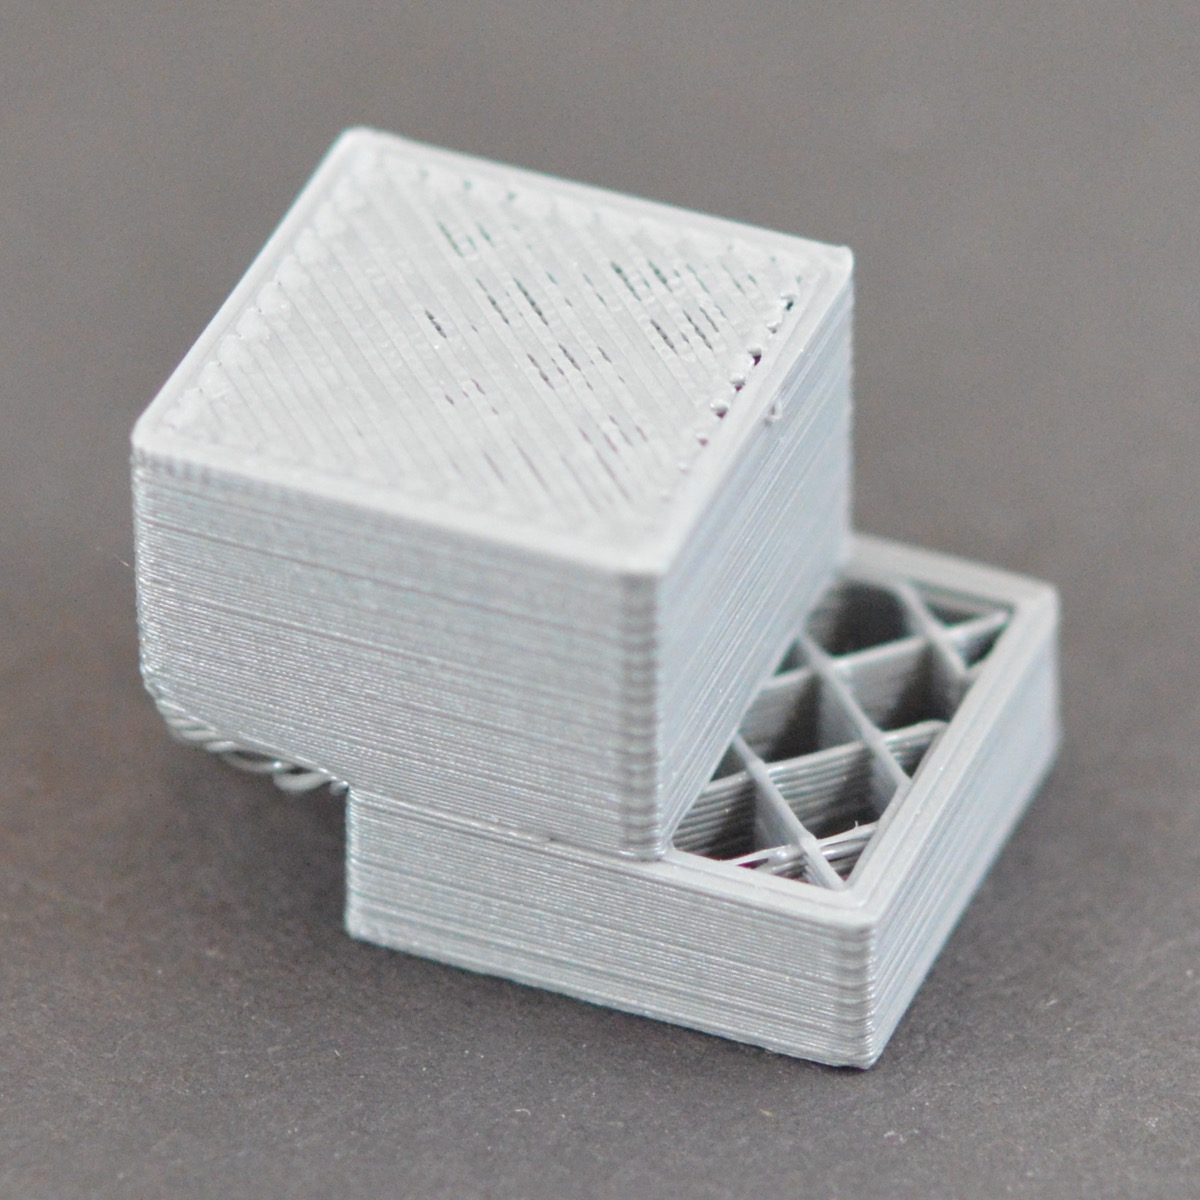
\includegraphics[width=\textwidth]{images/Layer-Shifting}
			\column{0.5\textwidth}
				\textbf{Desplazamiento de capa}
				\begin{itemize}
					\item Base mal asegurada
					\item Velocidad del cabezal demasiado alta
					\item Problemas mecánicos o electrónicos
				\end{itemize}
		\end{columns}
	\end{frame}
	\begin{frame}{Problemas comunes}
		\begin{columns}
			\column{0.5\textwidth}
				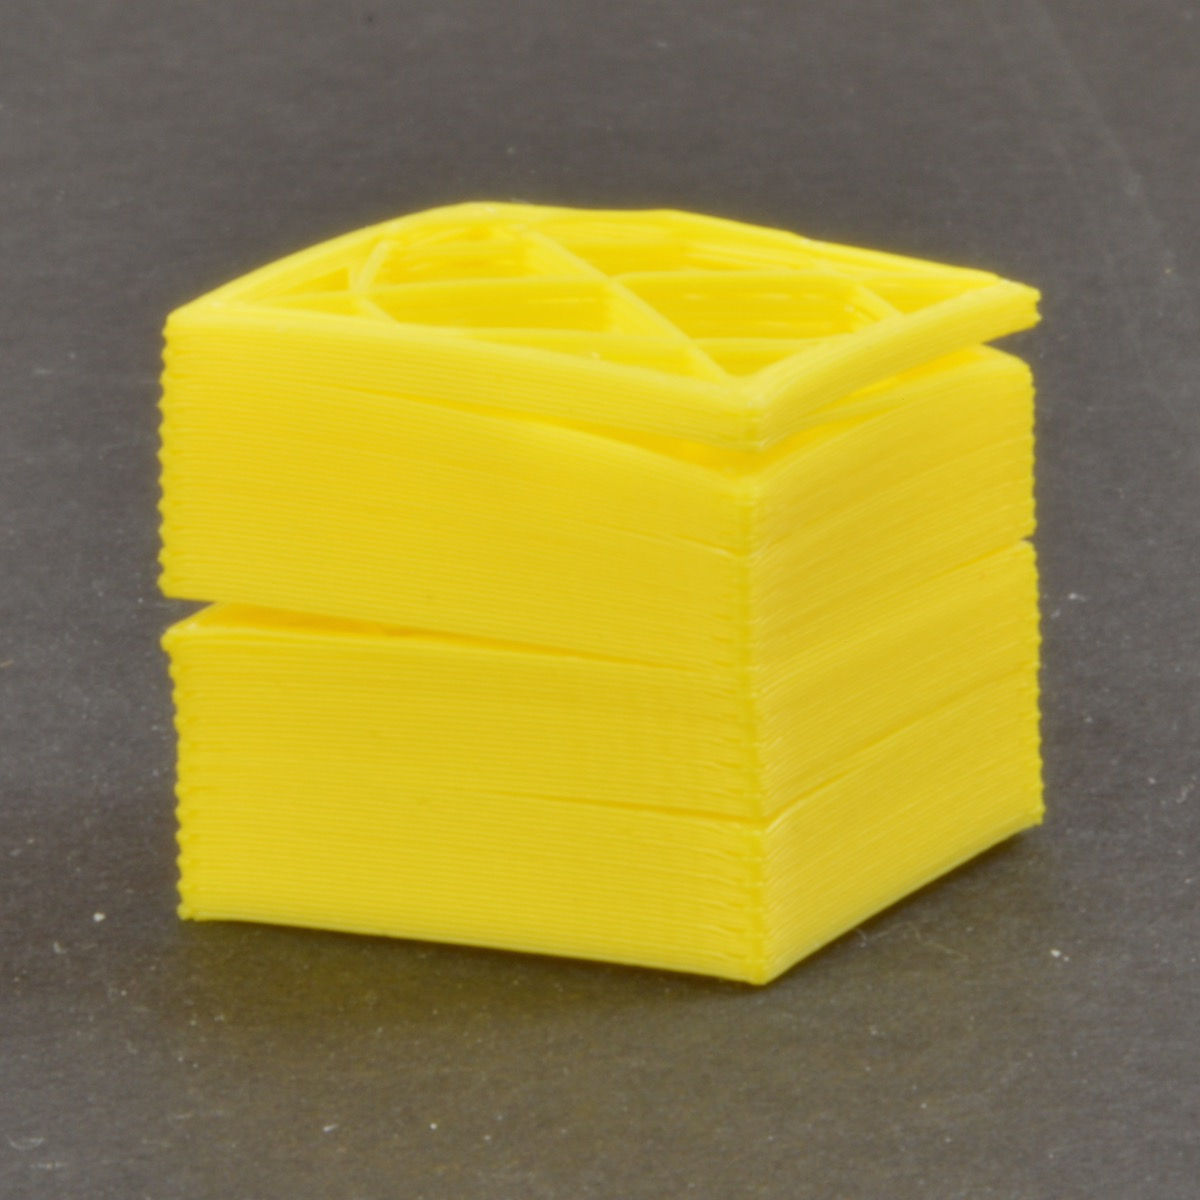
\includegraphics[width=\textwidth]{images/Layers-Splitting-Or-Cracking}
			\column{0.5\textwidth}
				\textbf{Separación de capa}
				\begin{itemize}
					\item Altura de capa demasiado grande
					\item Temperatura demasiado baja
				\end{itemize}
		\end{columns}
	\end{frame}
	\begin{frame}{Problemas comunes}
		\begin{columns}
			\column{0.5\textwidth}
				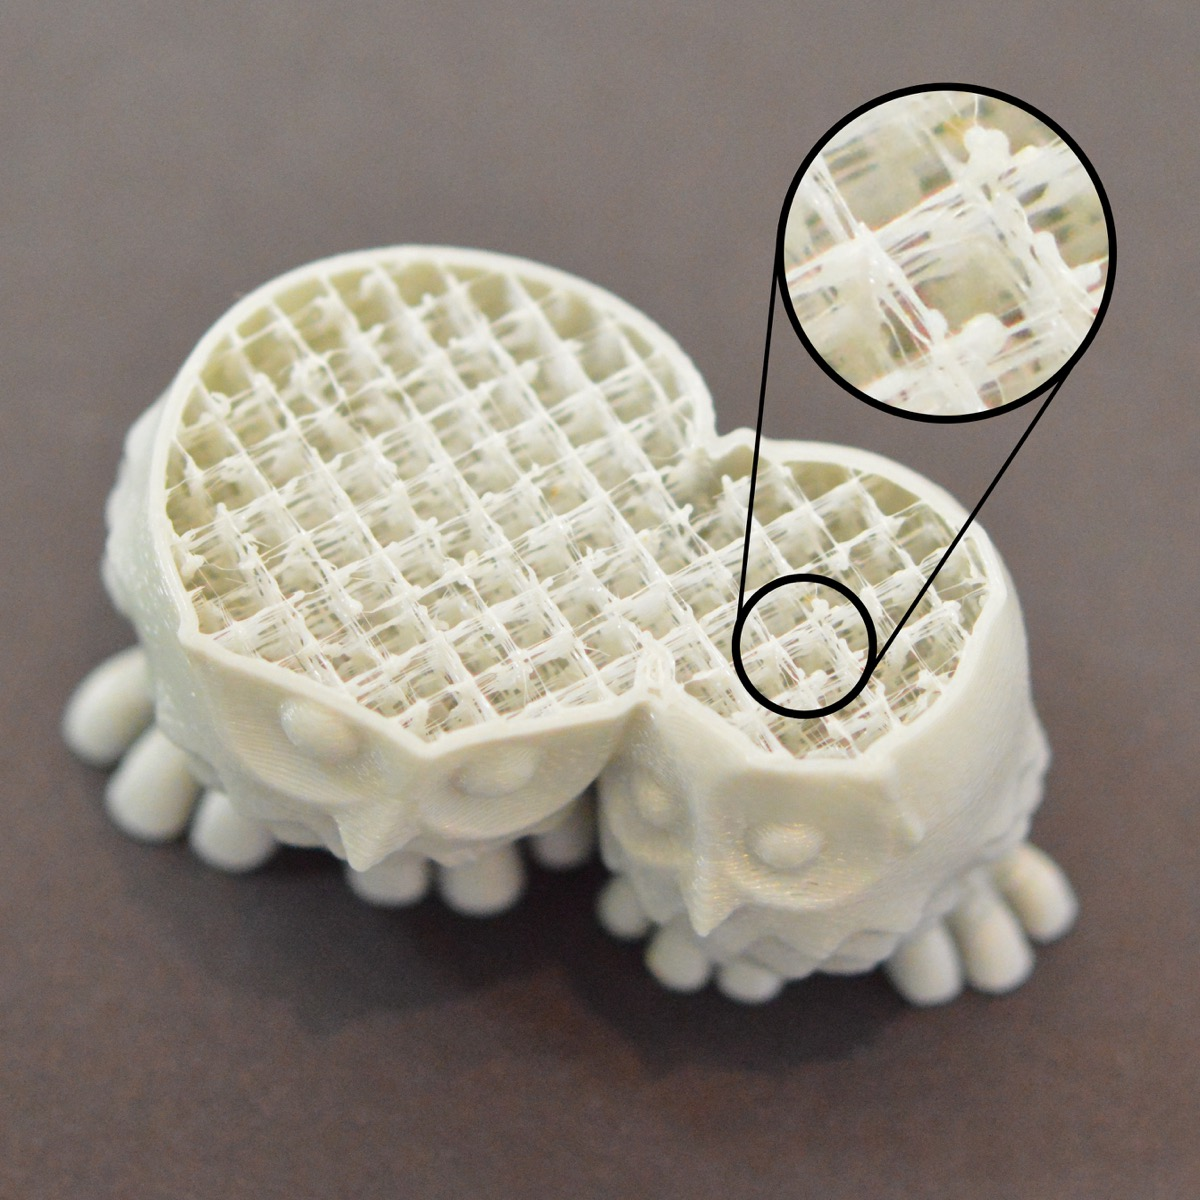
\includegraphics[width=\textwidth]{images/Weak-Or-Stringy-Infill}
			\column{0.5\textwidth}
				\textbf{Relleno débil}
				\begin{itemize}
					\item Cambiar patrón de relleno
					\item Bajar la velocidad de impresión
					\item Incrementar multiplicador de extrusión de relleno
				\end{itemize}
		\end{columns}
	\end{frame}
	\begin{frame}{Problemas comunes}
		\begin{columns}
			\column{0.5\textwidth}
				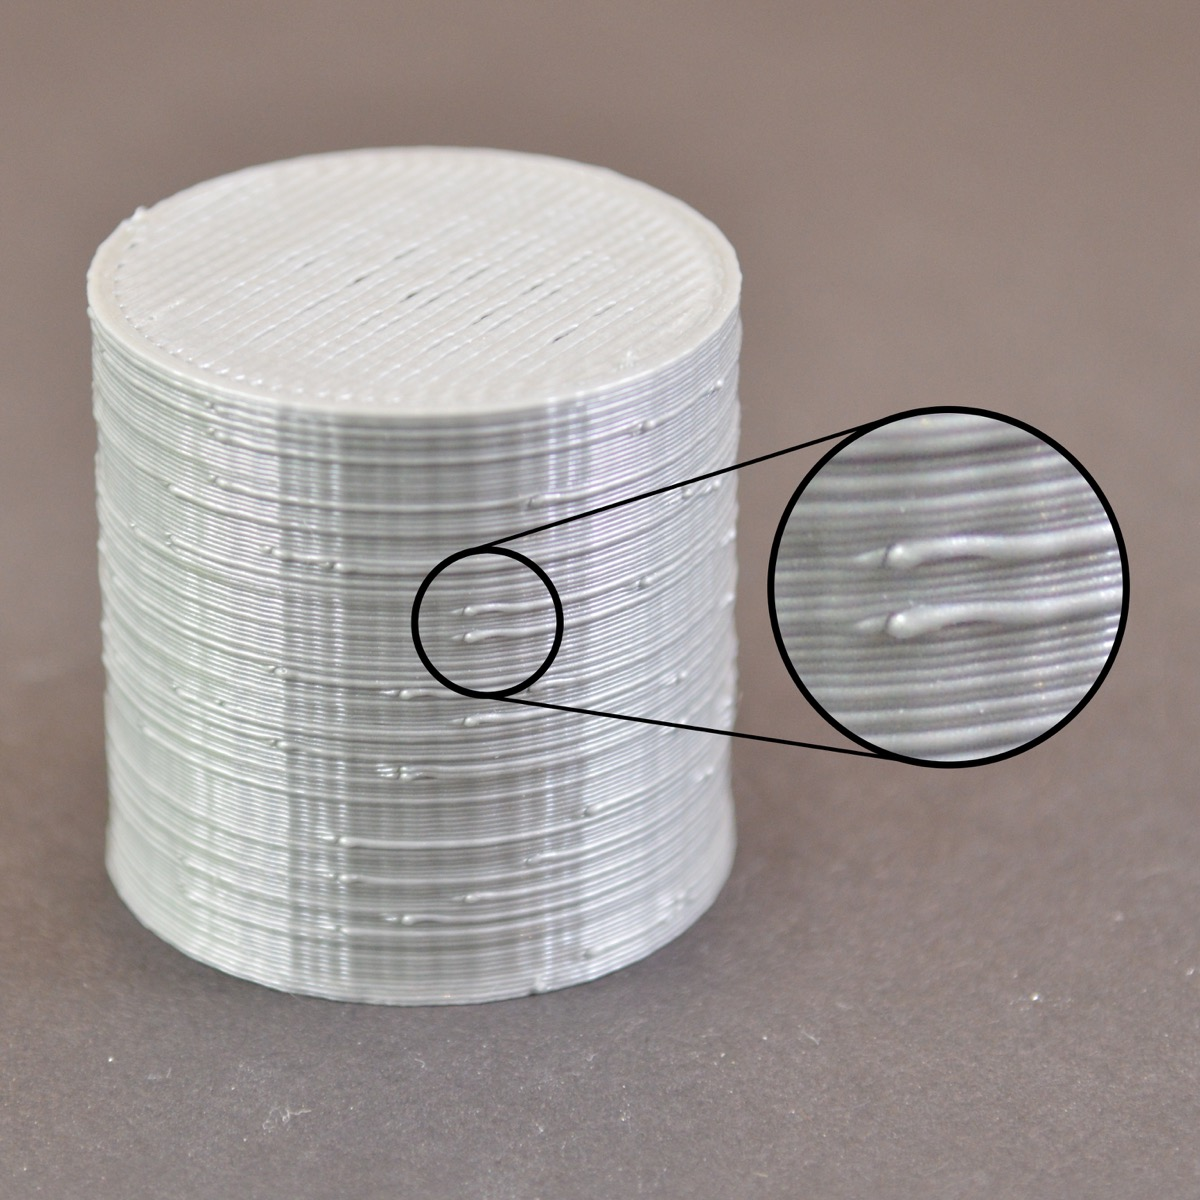
\includegraphics[width=\textwidth]{images/Blobs-And-Zits}
			\column{0.5\textwidth}
				\textbf{Gotas, manchas y bultos}
				\begin{itemize}
					\item Ajustes de retracción
				\end{itemize}
		\end{columns}
	\end{frame}
	\begin{frame}{Problemas comunes}
		\begin{columns}
			\column{0.5\textwidth}
				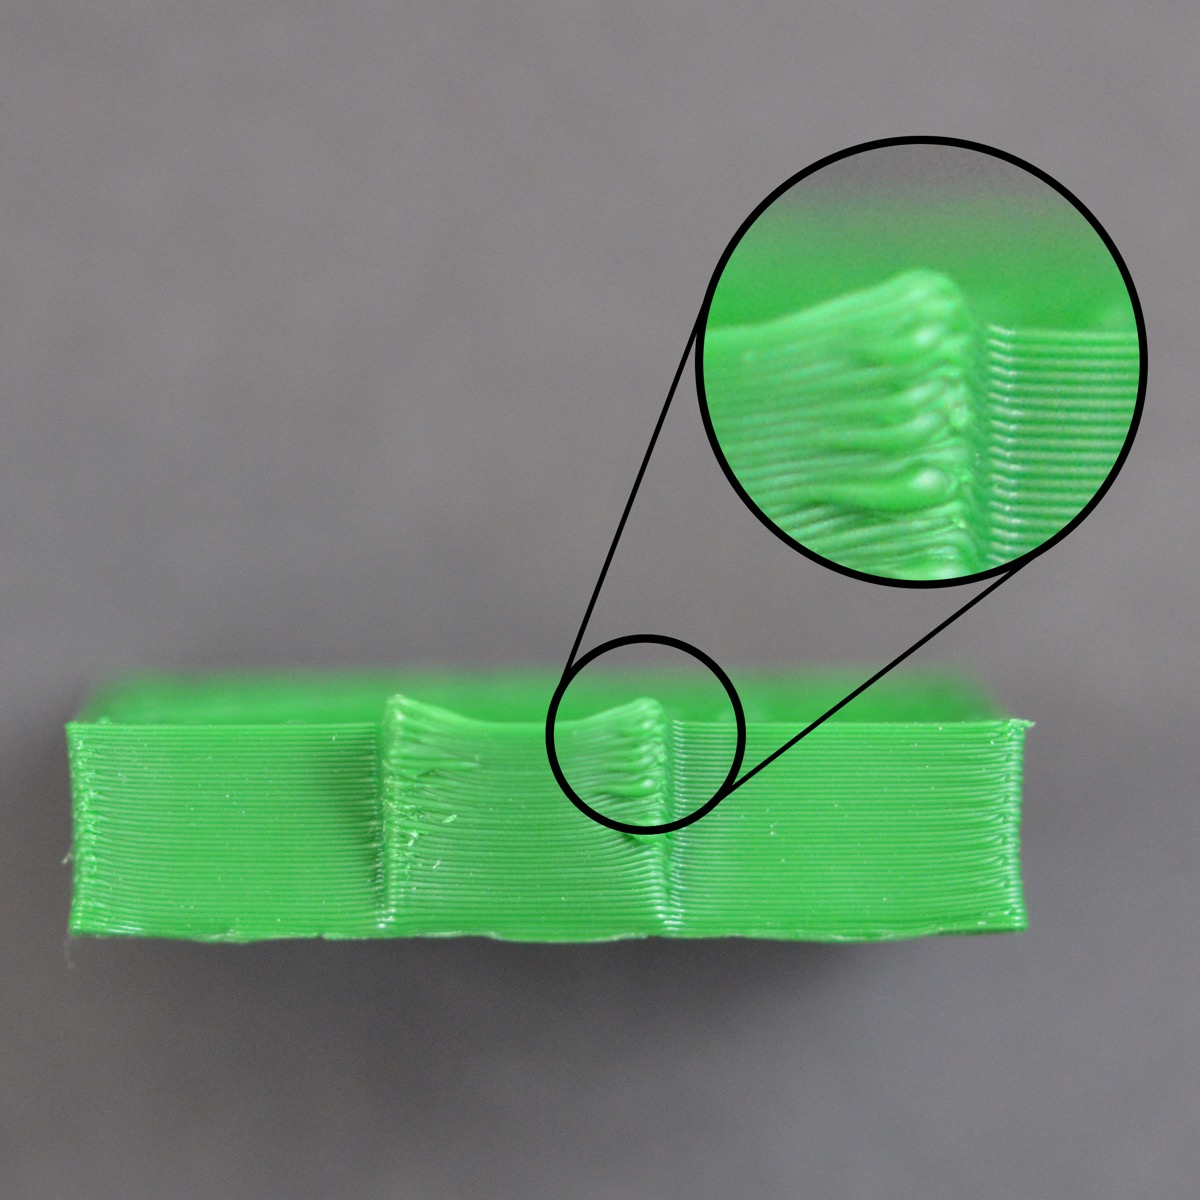
\includegraphics[width=\textwidth]{images/Curling-And-Warping}
			\column{0.5\textwidth}
				\textbf{Mala calidad en voladizos}
				\begin{itemize}
					\item Geometría de la pieza
					\item Reducir altura de capa
					\item Soportes
				\end{itemize}
		\end{columns}
	\end{frame}
	\begin{frame}{Problemas comunes}
		\begin{columns}
			\column{0.5\textwidth}
				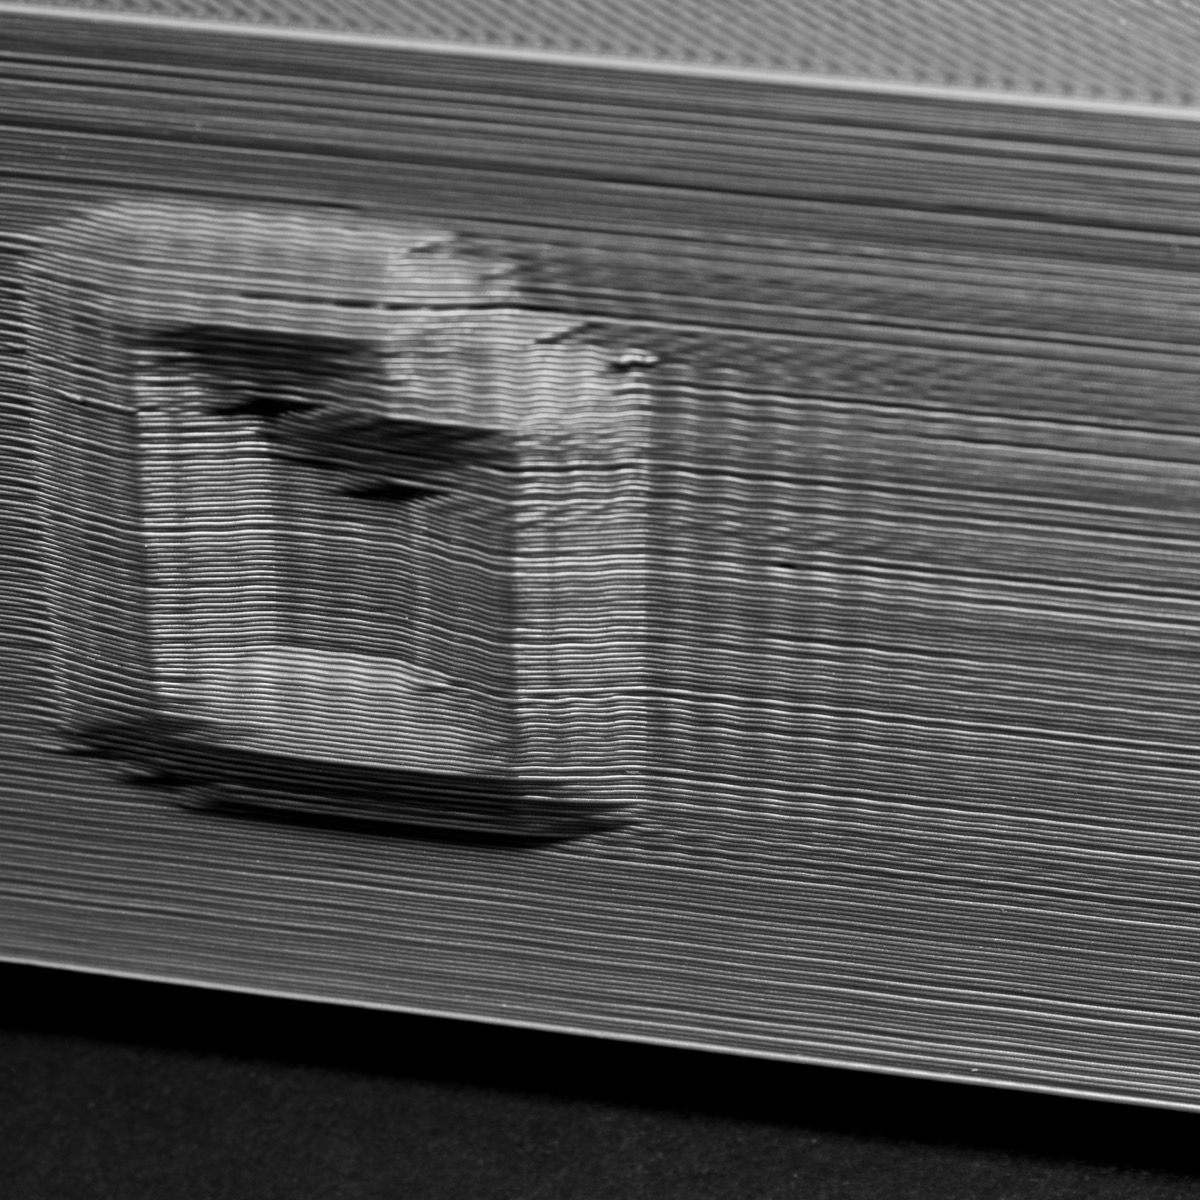
\includegraphics[width=\textwidth]{images/Vibrations-And-Ringing}
			\column{0.5\textwidth}
				\textbf{Vibraciones y reonancia}
				\begin{itemize}
					\item Reducir velocidad de impresión
					\item Reducir la aceleración
					\item Problemas mecánicos
				\end{itemize}
		\end{columns}
	\end{frame}
	\begin{frame}{Problemas comunes}
		\begin{columns}
			\column{0.5\textwidth}
				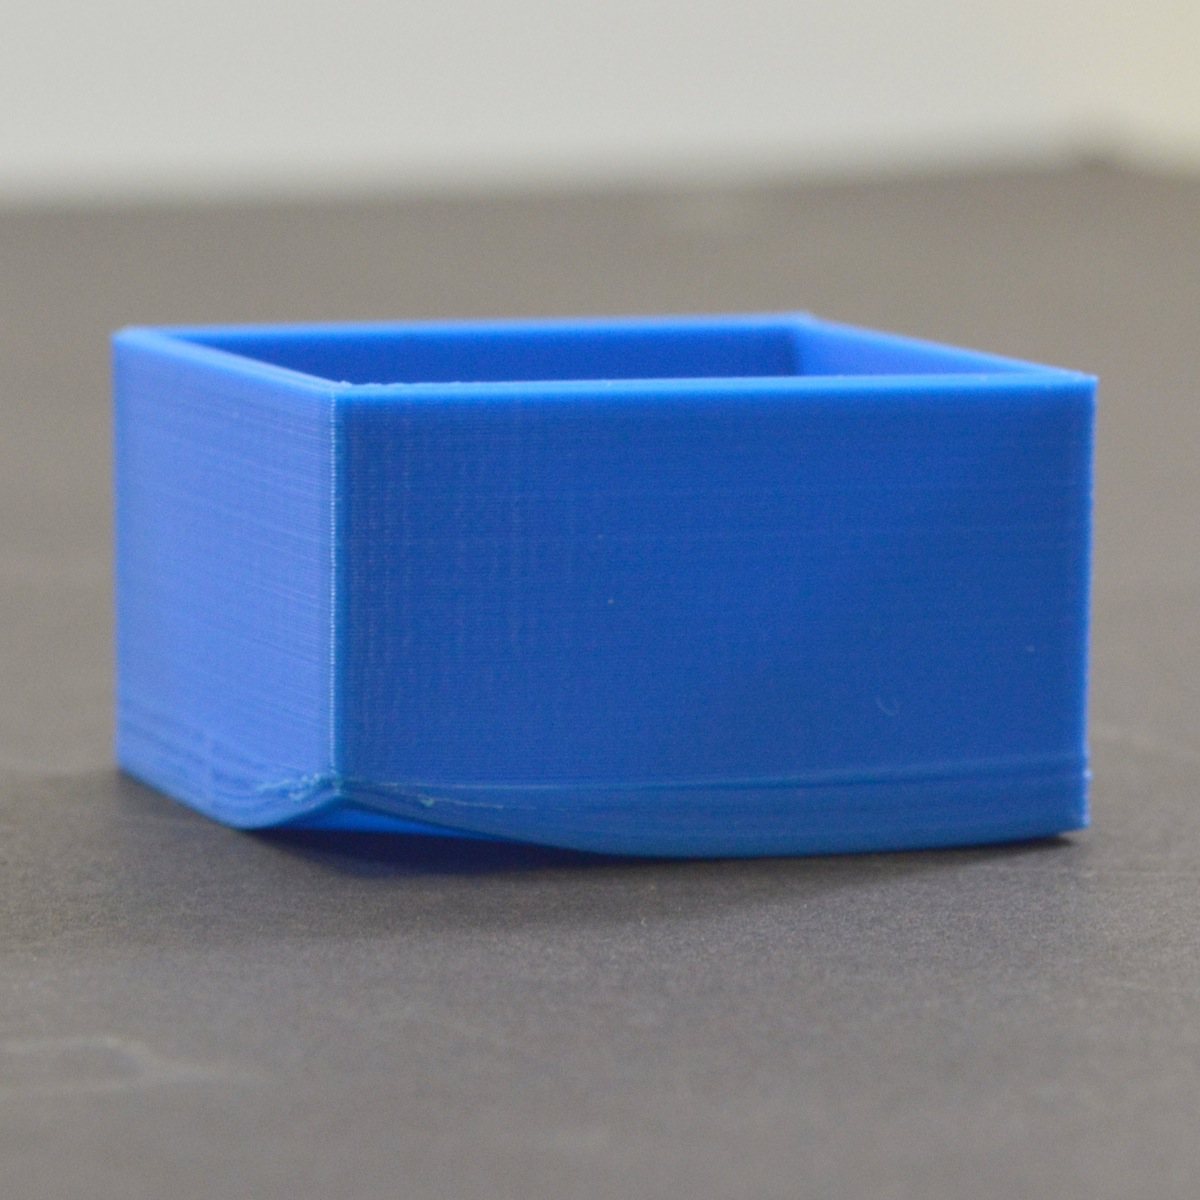
\includegraphics[width=\textwidth]{images/Warping}
			\column{0.5\textwidth}
				\textbf{``Warping''}
				\begin{itemize}
					\item Cama muy fría
					\item Cambiar adhesivo
					\item Disminuir la refrigeración
					\item Control de clima
					\item Bordes o balsa
				\end{itemize}
		\end{columns}
	\end{frame}
	
	%%%%%%%%%%%%%%%%%%%%%%%%%%%%%%%%%%%%%%%%
	\section{Tras la impresión}
	\begin{frame}{Extraer y limpiar la pieza}
		\begin{figure}
			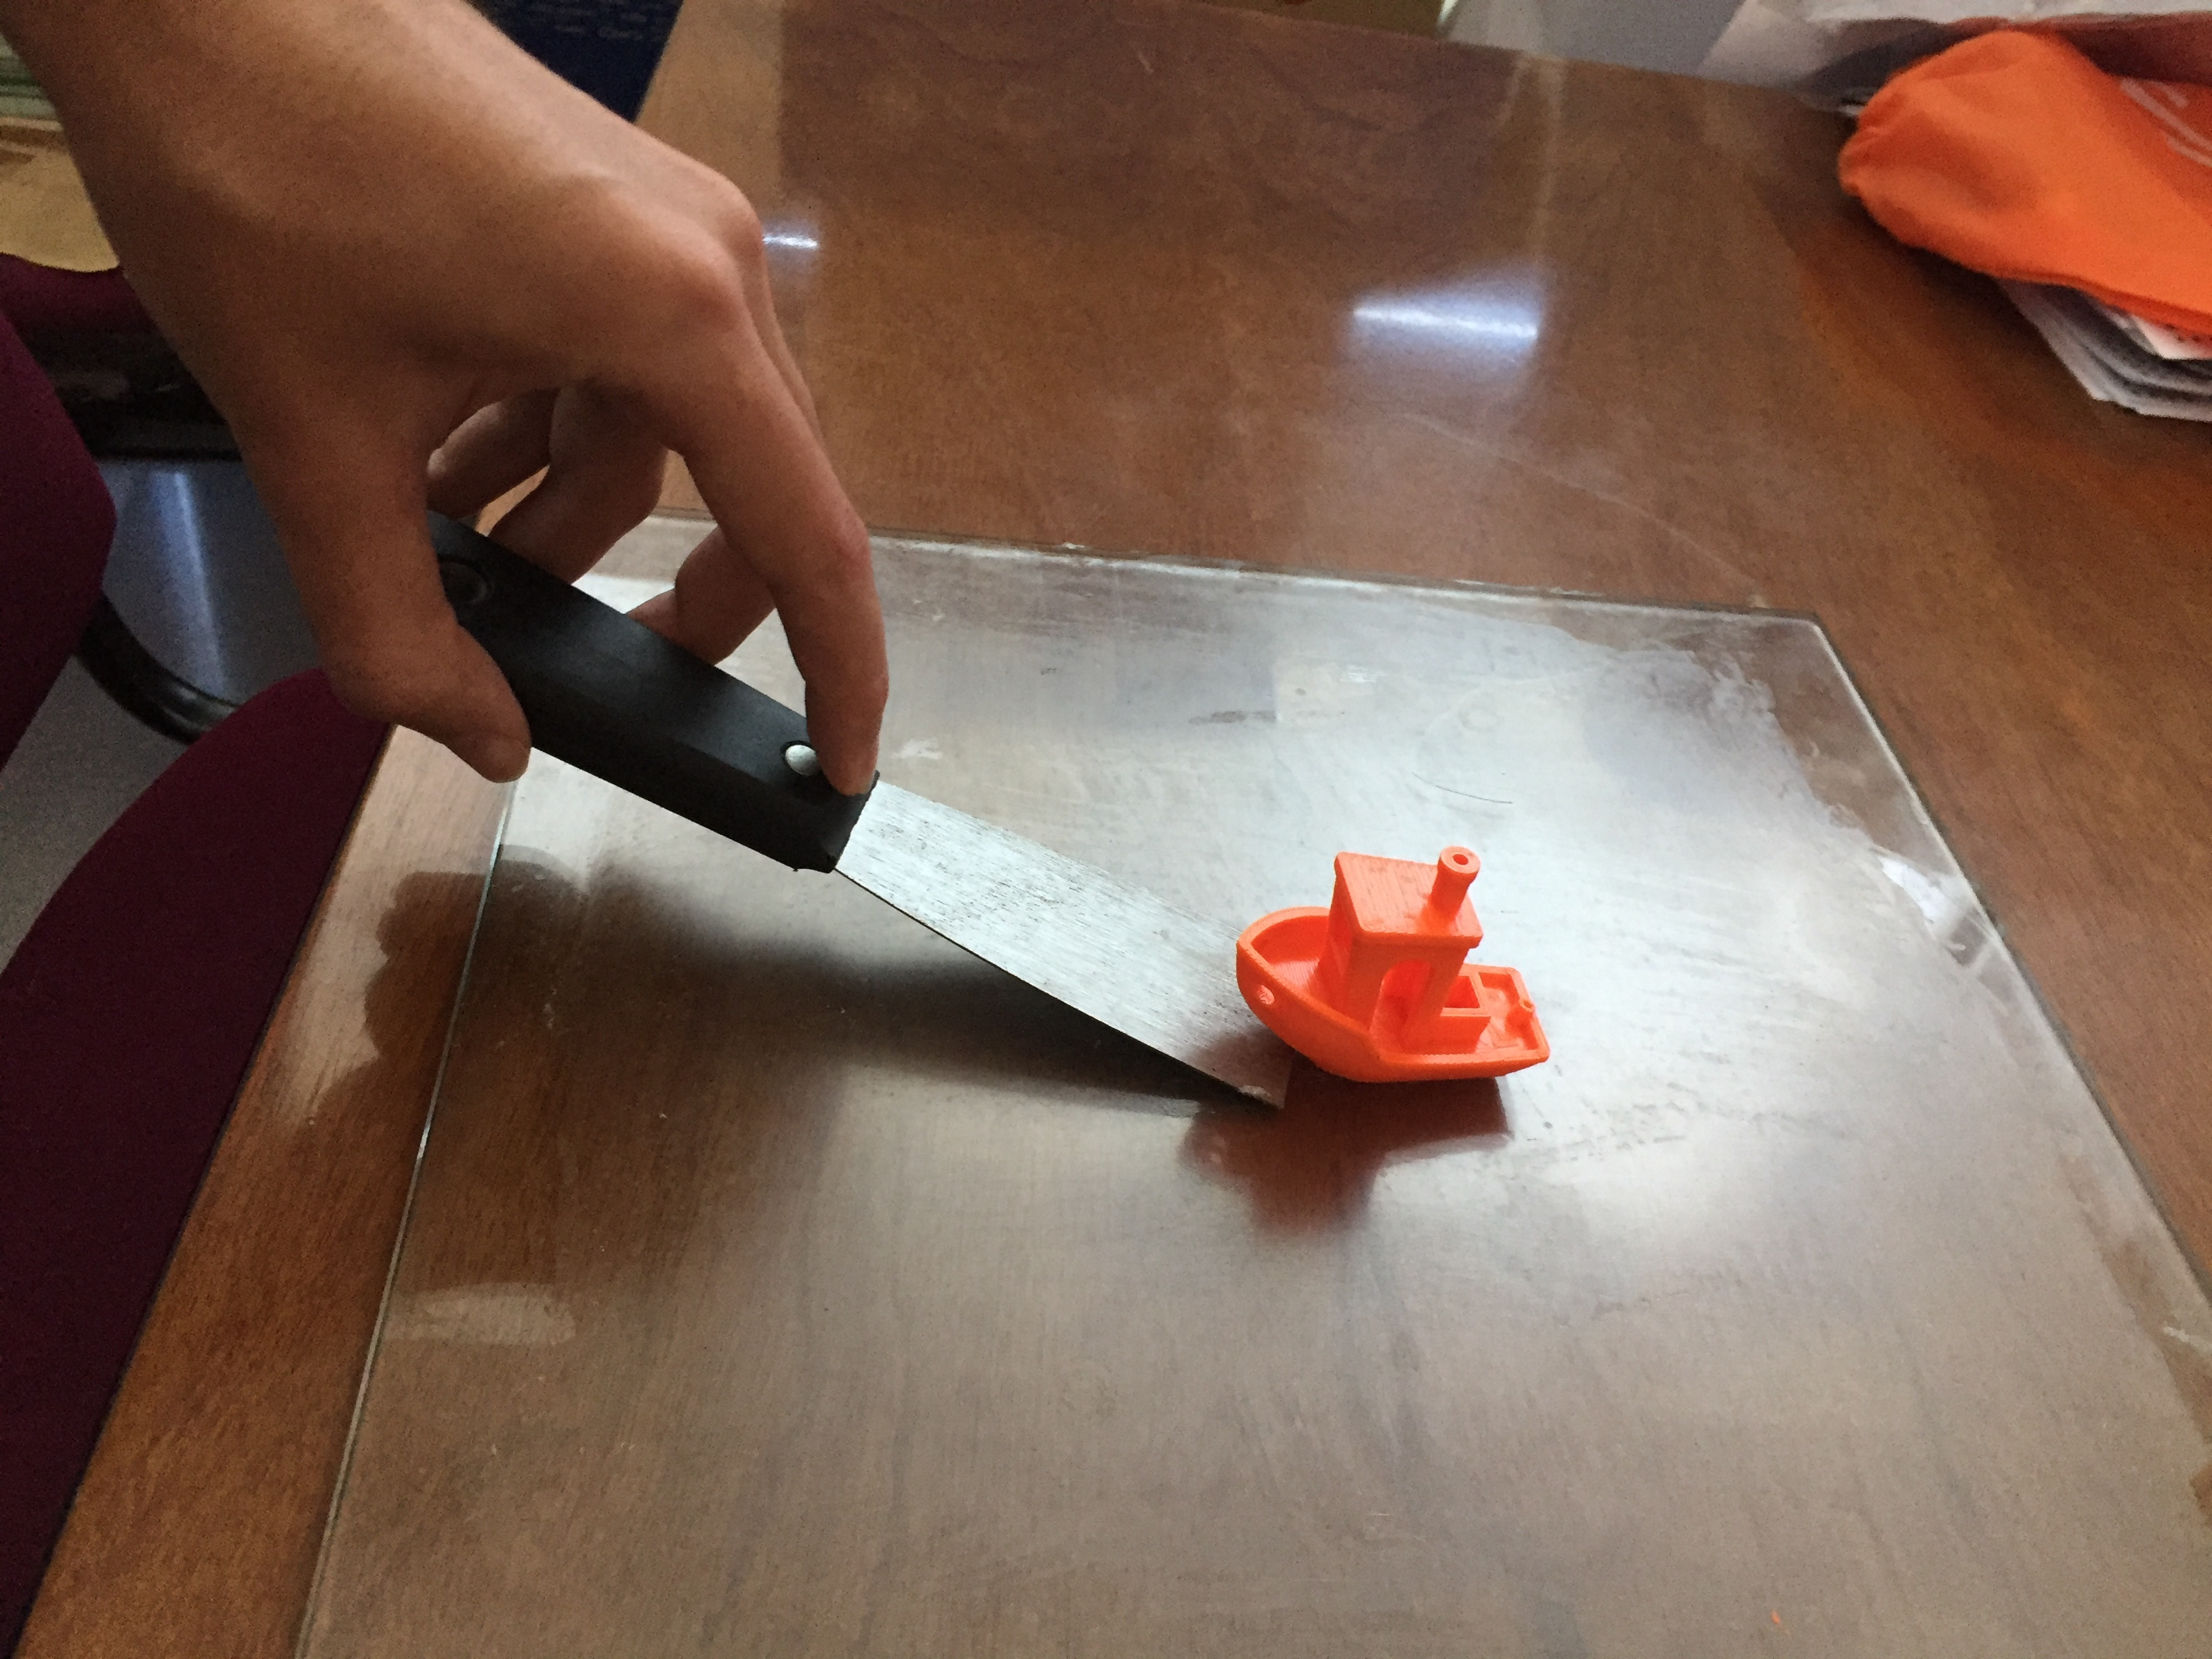
\includegraphics[width=.75\textwidth]{images/extraer}
			\caption{Utilizar una espátula y empujar}
		\end{figure}
	\end{frame}
	\begin{frame}{Post-tratamiento}
		\begin{figure}
			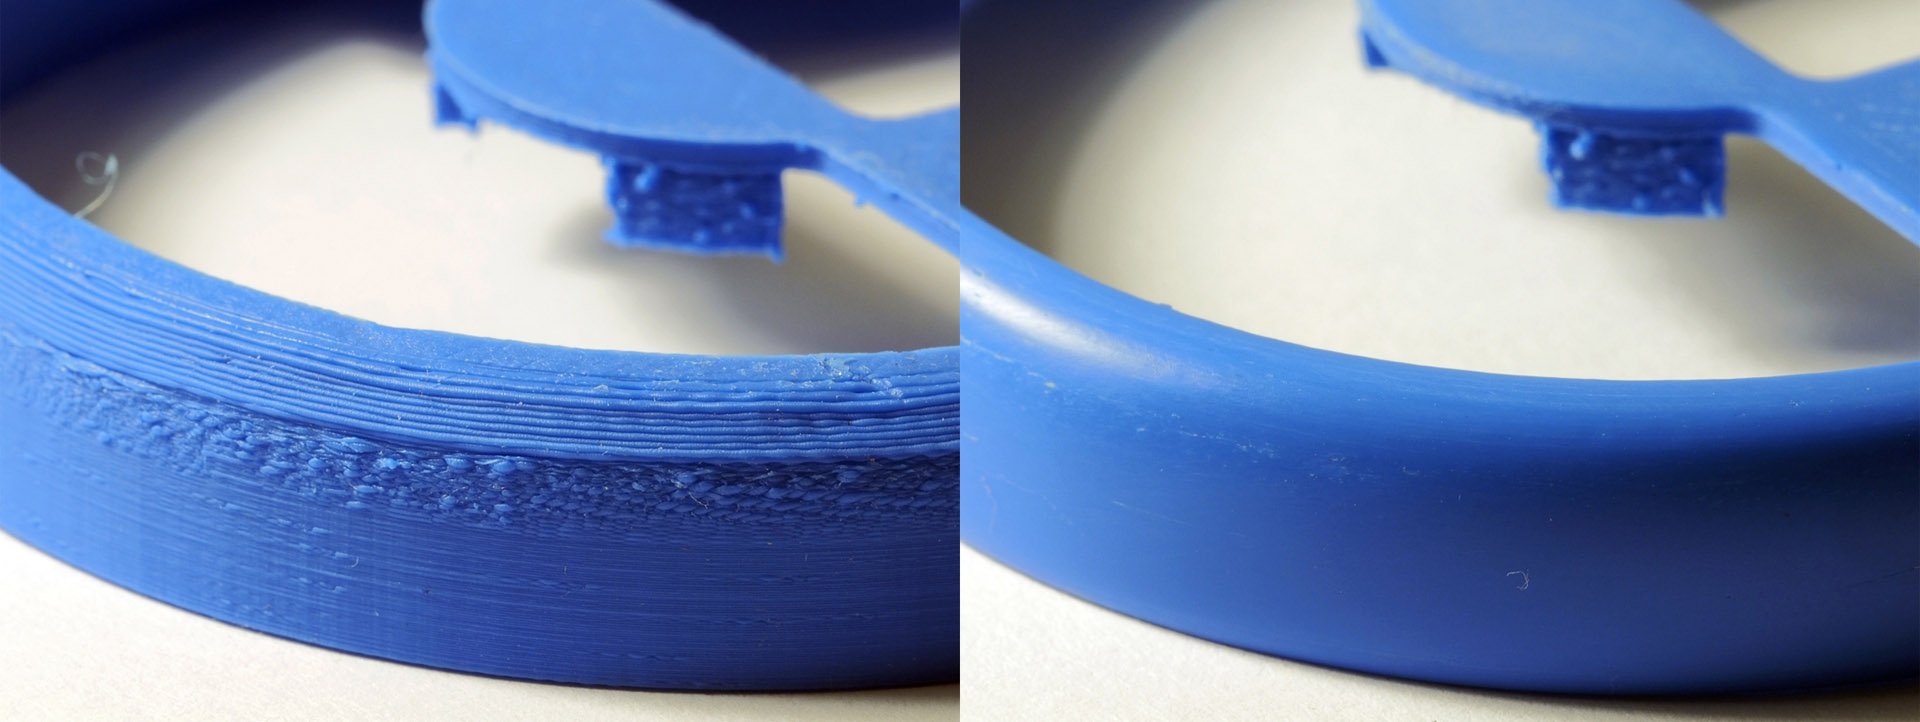
\includegraphics[width=\textwidth]{images/lijado}
			\caption{El lijado puede eliminar las marcas del proceso de fabricación}
		\end{figure}
	\end{frame}
	
	\begin{frame}[standout]{FIN}
		¡Felicidades, ahora sabes cuantos problemas puede dar la impresión 3D!
	\end{frame}
\end{document}
